\iffalse % CHANGE TO iffalse FOR RELEASE
\documentclass[letterpaper,10pt,oneside]{book}
\usepackage[compact]{titlesec}   % Reduce the space between titles and text
\titleclass{\chapter}{straight}
\titleformat{\chapter}[display]
  {\normalfont\huge\bfseries}{\chaptertitlename\ \thechapter}{20pt}{\Huge}
\titlespacing*{\chapter} {0pt}{50pt}{40pt}
\else
\documentclass[letterpaper,12pt]{book}
\usepackage{setspace}
\onehalfspacing
\fi


\usepackage{geo}
\usletter

\usepackage{times}                 % Times New font
\usepackage{pifont}                % Ding symbols (for Cloud9)
\usepackage{wasysym}               % For the bullets in the interpreter comparison (Chef)
\usepackage{multirow}              % Cells spanning rows in tables
\usepackage{xspace}
\usepackage[labelfont=bf]{caption} % Bold caption labels
\usepackage{wrapfig}               % Side figures without caption




%% Global definitions
\newcommand{\thesistitle}{Improving Scalability of Symbolic Execution for Software with Complex Environment Interfaces}

\newcommand{\codebit}[1]{\textsf{\footnotesize #1}}

%% Cloud9 definitions
\newcommand{\cnine}{Cloud9\xspace}
\newcommand{\cninesuffix}{cloud9}

%% Chef definitions

\newcommand{\chef}{\textsc{Chef}\xspace}

\newcommand{\cupa}{{\small CUPA}\xspace}
\newcommand{\hlpc}{{\small HLPC}\xspace}
\newcommand{\hlpcs}{{\small HLPC}s\xspace}

\newcommand{\nicese}{NICE\xspace}
\newcommand{\cutiepy}{CutiePy\xspace}
\newcommand{\commuterse}{Commuter\xspace}



%% PDF SUPPORT
%% -----------

\usepackage[hidelinks]{hyperref} % Add cross references inside the PDF
\usepackage[all]{hypcap} % Fix the jump position when clicking figure references

\hypersetup{
  pdftitle={\thesistitle},
  pdfauthor={Stefan Bucur}
}



\begin{document}

\date{}
\title{\thesistitle}
\author{Stefan Bucur \\ EPFL, Switzerland}

\maketitle

\chapter*{Abstract (German)}

To be determined.

\chapter*{Abstract}

Software testing is laborious, time-consuming, and prone to human error.  Symbolic execution is a promising technique for automating test case generation.  However, its scalability to real-world software is limited by the \emph{environment problem}, i.e., the reliance of the target program on external functionality provided through complex interfaces, which the symbolic execution engine ought to support.
%
The environment problem is challenging to attack systematically, as its manifestations depend on the nature of the environment interface and its implementation.

This thesis addresses two instances of the environment problem, which collectively cover a wide range of real-world software: (1) system software interacting with the operating system, and (2) high-level programs written in dynamic languages, such as Python, Ruby, or JavaScript.  The two instances exhibit opposite characteristics: while the operating system interfaces are typically stable and well-documented (e.g., POSIX), the specifications of dynamic languages are incomplete and unstable.

To address the environment problem for stable operating system interfaces, this thesis introduces Cloud9, a symbolic execution platform that provides an accurate and efficient model of the POSIX interface, as used by systems such as system utilities, web servers, or distributed systems.
%
Cloud9 relies on the insight that, for the purpose of testing, the operating system interface can be modeled as guest code on top of a set of basic abstractions: threads and processes, synchronization, and address spaces with shared memory. These abstractions need to be provided as primitives by the symbolic execution engine, while the rest of the model can be emulated as guest code.

For incomplete and unstable dynamic language semantics, this thesis introduces Chef, a platform for obtaining symbolic execution engines for interpreted languages by reusing their interpreters as executable specifications.  In Chef, the target program is bundled with the interpreter, running in a low-level (e.g., x86) symbolic execution engine, such that the aggregate system acts as a high-level execution engine for the program.
%
%% Chef automatically maps the low-level interpreter paths to high-level program paths by segmenting each low-level path into distinct high-level instructions.
%
To circumvent the complexity of symbolically executing the entire interpreter, this thesis introduces Class-uniform Path Analysis (CUPA), a heuristic for prioritizing paths that works by grouping paths into equivalence classes according to a coverage goal.

\noindent \textbf{Keywords:} Symbolic execution, program environments, systems software, interpreted languages.


\chapter*{Acknowledgments}

TBD

\tableofcontents
\listoffigures
\listoftables

\chapter{Introduction}
\label{ch:introduction}
\section{Problem Definition}

\subsection{Limitations of Software Testing}

%% Software testing is resource-hungry, time-consuming, labor-intensive, and prone to human omission and error.  Despite massive investments in quality assurance, serious code defects are routinely discovered after software has been released~\cite{redHatSecurityX}, and fixing them at so late a stage carries substantial cost~\cite{codeComplete}.

Software testing is resource-hungry, time-consuming, labor-intensive, and prone to human omission and error.  A lot of bugs escape quality assurance into production, where they cause disruptions and data loss. For instance, in 2014, there were 19 CVE vulnerabilities reported on average per day, and estimates show that software bugs cost the global economy more than \$300 billion in 2013.

The security implications driven by today's connected world amplify the problem, with the largest disasters making the headlines.

At the same time, resources invested in testing are peaking. In 2014, about a quarter of the entire IT budget in enterprises was allocated to software testing, which was the highest figure to that date.  On average, developer teams spend as much as half of their time doing testing and fixing bugs.

Facing this situation, organizations recognize that software testing is cumbersome.  In a recent survely, more than two thirds of the organizations questioned admitted they have difficulties determining relevant tests for their software and pointed at the lack of adequate tools to support that.

\subsection{The Promise of Automated Test Case Generation}

%% Existing automated techniques, like model checking and symbolic execution, are highly effective at uncovering corner-case bugs typically missed by human scrutinity and hand-written tests.  However, their adoption in industrial general-purpose software testing has been hampered by two main challenges: applicability and scalability.

%% First, real-world systems interact heavily with the environment (e.g., through system calls or library calls) and may communicate with other parties (e.g., over sockets, IPC, shared memory).  A practical automated testing tool must be capable of handling these interactions while maintaining soundness (no false positives) and completeness (no false negatives).

%% Second, path explosion---the fact that the number of paths through a program is roughly exponential in program size---severely limits the extent to which large software can be thoroughly tested.

Existing automated techniques, like model checking and symbolic execution, are highly effective at uncovering corner-case bugs typically missed by human scrutinity and hand-written tests.

Symbolic execution, in particular, is attractive for targeting complex real-world software. It works by systematically enumerating all execution paths through a program.  It is attractive for three attributes: thoroughness (eventually enumerates all execution paths), soundness (unlike static analysis, there are no false positives), and flexibility (selection of paths can be prioritized, makes it attractive for targeting complex real-world software).

However, its adoption in industrial general-purpose software testing has been hampered by the path explosion problem---the fact that the number of paths through a program is roughly exponential in program size.

An important dimension of path explosion is the proliferation of execution paths outside the scope of the program of interest (e.g., inside system calls or library calls).  Dealing with that is challenging, as naively discarding possible executions may reduce the coverage, while abstracting (modeling) them inside the symbolic execution engine can be a significant engineering task.  We collectively call this set of challenges the \emph{environment problem} of symbolic execution.

In this thesis, we address the environment problem for two important classes of software that collectively cover a significant fraction of the real-world software running today: (1) low-level systems making rich use of the operating system interface, and (2) programs written in interpreted languages.  By expanding the scope of symbolic execution, we enable for the first time effective automated test case generation on a wide range of systems, which we demonstrate can find bugs and generate high-coverage test suites.

%%%%%%%%%%%%%%%%%%%%%%%%%%%%%%%%%%%%%%%%%%%%%%%%%%%%%%%%%%%%%%%%%%%%%%%%%%%%%%%%

\section{Background}

%% Testing a program consists of exercising many different paths through it and checking whether they ``do the right thing.''  In other words, testing is a way to produce partial evidence of correctness, and thus increase confidence in the tested software.  Yet, due to the typically poor coverage one can get today, testing often turns into a mere hunt for bugs.

%% In practice, most software test harnesses consist of manually written tests that are run periodically; regression test suites provide an automated way of checking whether new bugs have entered the code~\cite{codeComplete}.  Such suites tend to be tedious to write and maintain but, once in place, they can be reused and extended.  In practice, the state of the art consists mostly of fuzzing, i.e., trying various inputs in the hope of finding bugs and improving test coverage.

\subsection{Symbolic Execution Primer}

In research, the state of the art consists of model checkers and automated test generators based on symbolic execution~\cite{dart,klee}.  Instead of running a program with regular concrete inputs (e.g., $x\!=\!5$), symbolic execution consists of running a program with ``symbolic'' inputs that can take on all values allowed by the type (e.g., $x\!=\!\lambda$, where $\lambda \in \mathbb{N}$).  Whenever a conditional branch is encountered that involves a predicate $\pi$ that depends (directly or indirectly) on $x$, state and execution are forked into two alternatives: one following the then-branch ($\pi$) and another following the else-branch ($\neg \pi$). The two executions can now be pursued independently.  When a bug is found, test generators can compute concrete values for program inputs that take the program to the bug location.  This approach is efficient because it analyzes code for entire classes of inputs at a time, thus avoiding the redundancy inherent in fuzzing.

\subsection{Path Explosion}

%% The {\em first challenge} for such tools is path explosion, as mentioned earlier.  One way to cope is to memoize the symbolic execution of sub-paths into test summaries that can be subsequently reused when the same sub-path is encountered again, as done in compositional test generation~\cite{godefroid:compdyntest}.  Alternatively, it is possible to use various heuristics to prioritize the most interesting paths first, as done in \klee~\cite{klee}.  Another approach is to execute symbolically only paths that are of interest to the test, as done in selective symbolic execution~\cite{s2e}.

The size of the symbolic execution tree is exponential in the number of branches. Loops and recursion make things worse, with the number of paths potentially being infinite.

Dealing with the path explosion is crucial in ensuring the scalability of symbex.

Existing approaches work by either \emph{prioritizing}, \emph{folding}, or \emph{abstracting} paths.

Prioritizing paths means to use heuristics for determining the paths to select next, and optionally discarding the rest (pruning).  Randomness and static-analysis based heuristics are the most popular.

Folding paths means joining their representation either when they join in the CFG, or compositionally by computing summaries of sub-paths and reuse them when encountered again.

Abstracting paths mean replacing the execution of a complex part of the program with a simpler model that can be reasoned about symbolically more easily.

Neither of the approaches works well in all cases. The first two approaches help reduce the number of paths, at the expense of making each path more complex and slower (the entire complexity of the program is still encoded in the symbolic expressions).  The last approach simplifies the complexity, but in most cases it has a high upfront cost of determining the model, and risks being unsound (hence introducing false positives).

\subsection{The Environment Problem}

%% The {\em second challenge} is mediating between a program and its environment, i.e., symbolically executing a program that calls into libraries and the OS, or communicates with other systems, neither of which execute symbolically.  One possible approach is to simply allow the call to go through into the ``concrete'' environment (e.g., to write a file)~\cite{dart,exe}; unfortunately, this causes the environment to be altered for \emph{all} forked executions being explored in parallel, thus introducing inconsistency.  Another approach is to replace the real environment with a symbolic model, i.e., a piece of code linked with the target program that provides the illusion of interacting with a symbolically executing environment.  For instance, \klee uses a symbolic model of the file system~\cite{klee}. Of course, real-world programs typically interact in richer ways than just file I/O: they fork processes, synchronize threads, etc.  

%% We originally viewed the building of a complete environment model as an engineering task, but our ``mere engineering'' attempt failed: for any functionality that, in a normal execution, requires hardware support (such as enforcing isolation between address spaces), the core symbolic execution engine had to be modified.  The research challenge therefore is to find the minimal set of engine primitives required to support a rich model of a program's environment. 

Employing the three approaches is difficult when the source of path explosion is the program environment.  For instance, a program making use of libraries or OS syscalls.

One can employ pruning and allow the environment calls to go ``concretely'' in the environment.  In particular, the environment can be shared with the host, but this causes it to be altered for all forked executions and introduce inconsistency.

Another approach is to abstract the system (either model linked with program, or built into the engine).  But this is challenging for any non-trivial runtime, such as an operating system with hundreds of system calls.  For instance, \klee uses a symbolic model of the file system, but real-world programs interact in richer ways than just file I/O: they fork processes, synchronize threads, etc.

%%%%%%%%%%%%%%%%%%%%%%%%%%%%%%%%%%%%%%%%%%%%%%%%%%%%%%%%%%%%%%%%%%%%%%%%%%%%%%%%

\section{Solution Overview}

In this thesis, we address the path explosion of symbolic execution of real-world programs with complex environment interfaces by attacking two representative instances of the problem: low-level system software making rich use of the OS interface, and programs written in high-level interpreted languages, such as JavaScript, Python, Lua, etc.  These two correspond to two different environment scenarios: in the former, the interface is standardized and rather fixed, while in the latter it is highly volatile.

We prototyped the two approaches in two systems: Cloud9 is a symbolic execution platform for POSIX systems, while Chef is a platform for obtaining symbolic execution engines for interpreted languages by plugging the interpreter.

\subsection{Cloud9: Modeling Operating System Abstractions}

Cloud9 addresses the environment problem for the POSIX interface by leveraging the insight that only three abstractions need to be built into the engine, while the others can be implemented as guest code with less effort.  It also relies on the fact that in a symbolic environment, performance is less important (which in the real world would have been taken up by caches and additional layers of complexity).  By finding this sweetspot, Cloud9 keeps the model complexity low (hence reduced maintenance and extension effort), while supporting faithful execution for a wide set of real-world software, ranging from system utilities to web servers and distributed systems.

\subsection{Chef: Using Interpreters as Executable Language Specifications}

Chef addresses the environment problem for high-level interpreted languages (the environment here is the semantics and set of libraries available in the language).  The semantics of these languages are complex and volatile, so building a symbolic execution engine by hand is tedious.

Our insight is that we can use the interpreter of the language as an executable language specification.  By plugging in the interpreter into a low-level engine, we execute the high-level program.

We deal with the path explosion problem by providing a system where the high-level and low-level strategies are decoupled and can be optimized independently for the testing goal.

\subsection{Circumventing Path Explosion with CUPA}

Orthogonal to the two techniques addressing the environment problem, we further improved the performance of symbolic execution across all range of applications with two techniques.

Class Uniform Path Analysis is a path prioritization heuristic that leverages the observation that path explosion tends to be clustered in the so called ``fork bombs'':  regions of code, where states accumulate and bias a global selection strategy.  Instead, CUPA groups the states into classes, and then selects classes uniformly, effectively containing the path explosion.

\subsection{Addressing Path Explosion through Massive Parallelization}

%% We pursue a complementary approach---{\em parallel symbolic execution}---in which we symbolically execute a program in parallel on a cluster, thus harnessing the machines into a ``distributed computer'' whose aggregate CPU and memory surpass that of an individual machine.  An alternative to a cluster-based approach would be to run a classic single-node symbolic execution engine on a Blue Gene-like supercomputer with vast shared memory and CPUs communicating over MPI.  Supercomputers, however, are expensive, so we favor instead clusters of cheap commodity hardware.

%% One way to parallelize symbolic execution is by statically dividing up the task among nodes and having them run independently.   However, when running on large programs, this approach leads to high workload imbalance among nodes, making the entire cluster proceed at the pace of the slowest node~\cite{parallelSymbex}.  If this node gets stuck, for instance, while symbolically executing a loop, the testing process may never terminate.  Parallelizing symbolic execution on shared-nothing clusters in a way that scales well is difficult.

%% The work presented here aims to address these three challenges.  Cluster-based parallel symbolic execution (\S\ref{sec:parsymbex}) provides the illusion of running a classic symbolic execution engine on top of a large, powerful computer.  Without changing the exponential nature of the problem, parallel symbolic execution harnesses cluster resources to make it feasible to run automated testing on larger systems than what was possible until now. Our work complements and benefits all tools and approaches based on symbolic execution.  We describe a way to accurately model the environment (\S\ref{sec:posix}) with sufficient completeness to test complex, real software, like the Apache web server and the Python interpreter.  We present the APIs and primitives that we found necessary in developing a true testing platform (\S\ref{sec:platform}).  We show how using these APIs enables, for instance, finding errors in bug patches by reproducing environment conditions which otherwise would have been hard or impossible to set up with regular test cases.

Parallel symbolic execution.

\subsection{Symbolic Tests for Encapsulating the Symbolic Execution Task}

The {\em third challenge} is using an automated test generator in the context of a development organization's quality assurance processes.  To take full advantage of the automated exploration of paths, a testing tool must provide ways to control all aspects of the environment.  For example, there needs to be a clean API for injecting failures at the boundary between programs and their environment, there must be a way to control thread schedules, and so on.  There should be a way to programmatically orchestrate all environment-related events, but doing so should not require deep expertise in the technology behind the testing tools themselves.

%%%%%%%%%%%%%%%%%%%%%%%%%%%%%%%%%%%%%%%%%%%%%%%%%%%%%%%%%%%%%%%%%%%%%%%%%%%%%%%%

\section{Thesis Roadmap}

The rest of the thesis is structured as follows: ...


%%% Local Variables: 
%%% mode: latex
%%% eval: (visual-line-mode)
%%% fill-column: 1000000
%%% TeX-master: "main"
%%% End:



\chapter{Related Work}
\label{ch:relatedwork}
There is substantial related work in the area of symbolic execution and formal methods in general.  In this chapter, we review the use of symbolic execution for automated test case generation (Section~\ref{sec:relwork:atcg}) and its applications on real-world software targets (Section~\ref{sec:relwork:targets}).  In particular, we focus on how previous work addressed the path explosion problem (Section~\ref{sec:relwork:pathexpl}).

%%%%%%%%%%%%%%%%%%%%%%%%%%%%%%%%%%%%%%%%%%%%%%%%%%%%%%%%%%%%%%%%%%%%%%%%%%%%%%%%
%%%%%%%%%%%%%%%%%%%%%%%%%%%%%%%%%%%%%%%%%%%%%%%%%%%%%%%%%%%%%%%%%%%%%%%%%%%%%%%%

\section{Symbolic Execution for Automated Testing of Commodity Software}

%% We review the most important symbolic execution-based tools.  The story is chronological, illustrating the advancements brought by each tool.

%% King~\cite{king:symbolic:2} described symbolic execution as a practical middle ground between testing a program with a set of concrete inputs and using formal correctness proofs.  The paper introduced EFFIGY, an interactive symbolic execution tool where developers manually step through paths and switch states in the execution tree.  However, the tool could only handle small programs written in a custom language supporting basic integer operations, and had limited performance, due to limited solver capabilities.

Symbolic execution was introduced almost four decades ago as a test case generation technique~\cite{king:symbolic:2, boyer:symbolic}.  The first tools worked on domain-specific languages, supported basic numeric operations, and were mostly used for interactive debugging.  The effectiveness of the technique on more complex programs was limited by the lack of efficient and expressive constraint solvers and slow hardware.

%% It was only in the past decade that symbolic execution has become a feasible approach to test generation for real-world software, with the advent of modern constraint solvers, such as Chaff~\cite{chaff}, MiniSAT~\cite{minisat}, STP~\cite{stp}, Z3~\cite{Z3}, or CVC~\cite{cvc}, and the exponential increase in hardware performance.  Our tools build on this foundation, too---both Cloud9 and Chef resort to the STP solver for all symbolic queries, such as branch feasibility checks.

The exponential increase in hardware performance and the availability of fast off-the-shelf constraint solvers~\cite{chaff,minisat,stp,Z3,cvc} amplified the research in symbolic execution.  Over the past decade, the new crop of symbolic execution engines generated test suites and found bugs on real-world software ranging from small system utilities to large application suites.

In this section, we highlight the most important tools and position \cnine and \chef with respect to them.

\subsection{System-level Software Targets}

%% \paragraph{DART}

%% DART automatically extracts the environment interface of a C program using static analysis.  DART augment the classic random fuzzing with a dynamic analysis that collects. The advantage of concrete execution is that DART can fall back on concrete semantics when symbolic ones are not supported (e.g., multiplications) DART detects standard errors such as crashes, assertion violations, and hangs.  Dart extracts the static interface of a program, consisting of global variables and inputs to the program entry function.  It concretizes calls to library functions.

%% Initializing values in DART: either randomly, or NULL or malloced values (for pointer types).  Chef and Cloud9 leaves it to the symbolic test the job of creating inputs. The basic primitives are marking allocated buffers (or integers or strings) as symbolic.
%% Dealing with environment inconsistencies in DART: Not a problem, as programs are re-executed (so no cross-talking in paths).  But assume no side effects in the program.
%% Solver in DART: lp\_solve (linear constraints of integers and reals).
%% DART was applied on C benchmarks and an implementation of the SIP protocol, finding hundreds of crashes.
%% DART uses DFS, BFS, or random.

%% \paragraph{CUTE}
%% Unit testing using concolic execution, with memory graphs as inputs.  Separates memory constraints from scalar constraints and keeps pointer constraints simple to keep the decision procedure tractable and efficient.
%% CUTE uses DFS.
%% CUTE uses its own in-house solver, built on top of lp\_solve, which adds optimizations such as incrementality.
%% CUTE supports generation of structured data by either calling sequences of operations, or solving data structure invariants (repOk operations), similar to Korat~\cite{boyapati:korat}.
%% Used for testing data structures.

\paragraph{Concrete + Symbolic Execution}

Targeting system software using symbolic execution is challenging, as the engine should support all program constructs, as well as the calls the program makes into its environment.
%
A solution adopted by early engines, such as DART~\cite{dart} and CUTE~\cite{cute}, was to instrument the original C source of the program, using tools such as CIL~\cite{cil}, with additional statements that maintain the symbolic state as the program executes.  This approach resulted in the so called \emph{concolic} (\emph{conc}rete + symb\emph{olic}) execution model, where the program executes normally with a concrete input, while collecting constraints for each branch taken, used to generate a new input for a new execution.
%
Whenever the symbolic execution was not supported, such as when dealing with external library calls, the program would simply stop collecting constraints and execute concrete-only.
%
Using this approach, DART and CUTE found crashes in C programs, such as protocol implementations and data structure libraries.

%% \paragraph{EXE}
%% Dedicated constraint solver STP, codesigned with EXE, optimized for reasoning about bitvectors and arrays, which accurately encode machine operations at good performance.
%% Has a flat view of memory.
%% Works by translating the C code to an instrumented format that includes checks for concrete/symbolic values, forks (UNIX forks), and checks for properties (memory errors, division by zero).
%% Introduced constraint optimization: caching, constraint independence.
%% DFS/BFS as search heuristics.
%% Found bugs in udhcpd, packet filters (BPF), pcre regexp library.

\paragraph{Specialized Solver Support}

In addition, non-trivial software also generates constraints that are hard to reason about, containing expressions such as memory accesses with symbolic addresses, or complex arithmetics such as bit-wise multiplications and divisions.  Without solver support, a symbolic execution engine needs to concretize the state or abandon the path, hence losing completeness.

To address this problem, modern symbolic execution engines employ off-the-shelf constraint solvers, such as Z3~\cite{Z3}, STP~\cite{stp}, or CVC~\cite{cvc}.  These solvers can reason efficiently about a large set of operations commonly encountered in program execution, such as bit-wise arithmetic and array access.
%
The EXE~\cite{exe} symbolic execution engine was among the first to employ such a solver (STP), co-designed with the symbolic execution engine to accurately express machine operations in languages such as C.
%
For example, EXE modeled the program memory as a flat array of bytes, with support for arbitrary pointer reads and writes, mixed with fixed-width integer operations.
%
As a result, EXE found bugs in system software such as the \codebit{udhcpd} DHPC server, packet filters, and the \codebit{pcre} Perl regular expression library.

\paragraph{Low-level Symbolic Interpretation}

Implementing symbolic execution semantics through source code instrumentation becomes difficult for large software with multiple units, or for more complex languages, such as C++.
%
As a result, the most recent (and most successful) symbolic execution engines target the lower-level compiled representations of programs, such as x86 binary or LLVM~\cite{llvm} bytecode~\cite{godefroid:fuzz,klee,bitBlaze,s2eSystem,mayhem}.  These representations consist of a smaller set of simpler instructions that are well specified and relatively stable.

%% \paragraph{SAGE}~\cite{sage2012,godefroid:fuzz}
%% Used in production, during Windows development, found thousands of vulnerabilities.  Largest known deployment of symbolic execution in production.
%% Targeted large applications, binary-level.
%% Introduces the generational search heuristic for finding bugs more efficiently in an incomplete search.

%% SAGE~\cite{sage2012,godefroid:fuzz} is the most successful use of symbolic execution in production.  It relies on concolic execution done at binary (x86) level.  It targets large applications with deep execution paths, such as Windows format parses and Microsoft Office applications.  To effectively explore the large search space, SAGE introduced a generational search heuristic.  The idea is to start from a concrete input that takes the program down a relevant path (e.g., a valid Office document), then alternate all branches on that path, then do the same with the second-generation inputs (hence the ``whitebox fuzzing'' name).
%% %
%% SAGE found thousands of Windows vulnerabilities at development time.

For example, SAGE~\cite{sage2012,godefroid:fuzz}---the most successful use of symbolic execution in production---performs concolic execution at binary level.
%
SAGE targets large applications with deep execution paths, such as Windows format parsers and Microsoft Office applications.
%
SAGE found thousands of Windows vulnerabilities at development time.

%% \paragraph{KLEE}
%% Uses symbolic execution for testing real-world systems code (Coreutils, Hi-star kernel, Busybox).  They built a high-performance symbolic execution engine that finds bugs in highly tested code and achieves high coverage levels.
%% Compact state representation using COW.
%% Uses a high-performance SMT solver (STP), and optimizes interface to the solver (constraint caching, expression simplifications).
%% Handles the environment problem through a model of files (used by the Coreutils), and external calls into the host environment.
%% Handles C code by compiling and running LLVM.
%% Uses static heuristics to maximize coverage, plus standard strategies.
%% Command line interface for marking inputs symbolic.

%% To target systems of increasing complexity, symbolic execution engines needed to address the environment problem.
%% %
%% KLEE~\cite{klee} was the first symbolic execution engine to target system software that communicates with its environment.  KLEE provides robust support for complex system software by having the software compiled to LLVM~\cite{llvm} IR, which is then interpreted symbolically.
%% %
%% KLEE~\cite{klee} introduced environment models as approximations of the real OS interface: the models replace parts of the standard C library and provided support for files.
%% %
%% This resulted in KLEE uncovering crashes and generating test suites with over 90\% coverage on average in the popular Coreutils utilities (e.g., \codebit{ls}, \codebit{echo}), testing Busybox and an OS kernel.
%% %
%% Our Cloud9 system builds on top of KLEE, providing symbolic primtives for a large fraction of the POSIX interface, as well as adding support for parallel symbolic execution.

KLEE~\cite{klee} is currently the most popular symbolic execution engine.  It is openly available and has served as a basis for a wide range of other tools.
%
KLEE works as a symbolic interpreter for LLVM IR bytecode, obtained by compiling source programs using an LLVM-based compiler such as Clang.
%
KLEE tackles the environment problem by introducing \emph{models} that approximate the real OS interface.  The KLEE models replace parts of the standard C library and provide basic support for file operations.  Unmodeled system calls are passed on to the host environment, executed concretely on behalf of the KLEE process.
%
KLEE found bugs and generated test suites with over 90\% statement coverage on average in the popular Coreutils suite.  It also found bugs in other systems software, such as Busybox and the HiStar kernel.

Modeling the environment is not always feasible.  In some cases, a component is so deeply integrated in the system that there is no clear separation between the component and the rest of the system.  Device drivers running in OS kernels are one notable example.
%
For those cases, an alternative approach to the environment problem is to bundle the program, together with all its dependencies, in one large unit executed symbolically.

S2E~\cite{s2eSystem} takes this approach by providing a full virtual machine x86 symbolic execution environment, which includes programs, libraries, the operating system, and the hardware.
%
This allows S2E to accurately run ``in-vivo'' any part of the software stack, without the need of the source code.
%
Most notably, S2E discovered vulnerabilities in several Windows device drivers, some of whom were Microsoft-certified~\cite{ddt}.

%% \paragraph{AEG}~\cite{aeg}
%% Automated testing with the specific purpose of generating proofs of vulnerabilities (exploits), i.e., inputs that explicitly hijack the program control flow and get a shell.
%% Takes as input LLVM + binary, produces exploit.
%% Generated 16 exploits on 14 open-source projects.
%% Buggy path-first heuristic: When a path has a bug (unexploitable), it is likely that it'll exhibit more bugs that could be exploitable.
%% Loop exhaustion strategy: prioritize paths exploring maximum number of iterations.
%% Symbolic files: simplifies KLEE's interface.
%% Symbolic sockets: supplies fresh symbolic data.
%% Environment variables (concrete values, fully symbolic, failures).
%% Network, multithreading, formatting functions (about 70 system calls).  Not clear how sound the support is, nor what happens when a syscall is not supported.

%% \paragraph{Mayhem}~\cite{mayhem}
%% Finds 29 exploitable vulnerabilities in Linux and Windows programs.
%% System designed to handle efficiently (at the expense of completeness) large state spaces generated by large programs.  Efficient reasoning about symbolic memory (symbolic writes are concretized, symbolic reads are replaced with nested ite expressions).
%% Uses only binaries (no debug info needed).

%% \paragraph{Bitblaze}~\cite{bitBlaze}
%% Unified binary analysis platform, used mainly for malware analysis.


Symbolic execution also found use in security testing~\cite{aeg,mayhem,bitBlaze}.  For this task, reaching vulnerabilities is more important than achieving completeness, so engines in this space resort to simplifications to increase performance and reach deeper executions in larger programs.
%
For example, the AEG~\cite{aeg} tool uses symbolic analysis to both find bugs and automatically generate exploits (get a shell) from the bugs.  AEG uses heuristics that prioritize buggt paths and employs simple operating system models that minimize path explosion.
%
The Mayhem~\cite{mayhem} tool employs a simplified symbolic memory model where write addresses are concretized.
%
Both tools found exploitable vulnerabilities in Linux and Windows programs.

%% Handling real-world targets: C, C++ (KLOVER), parallel systems (explain the two ways to run these systems symbolically, depending on what bugs we're looking for).

\subsection{Virtual Machine-based Languages: Java and C\#}

%% \paragraph{Java Path Finder}
%% \cite{jpf-symbex,jpf-testgen,generalized-symbex}.
%% Code that manipulates complex data structures.  Uses lazy initialization to instantiate data structures.
%% Built on top of the JVM.
%% Uses iterative deepening combined with DFS.
%% Model checking as a form of testing: since the program environment is typically way too large, model checking ends up being testing.
%% Can be used to either execute a repOk method and generate blackbox inputs, or do whitebox testing.

%% \paragraph{Pex}
%% Pex~\cite{tillmann-pex}.
%% Whitebox fuzzing for .NET.  Integrated in Visual Studio.  Found errors in a core .NET component.
%% Uses PUTs (parameterized unit tests)~\cite{tillmann-puts}.
%% Uses a ``meta-strategy'' that groups branches in equivalence classes, and then selects the lest chosen class.  Different sets of equivalence classes are chosen uniformly.
%% Constructing objects: run symbolically the object constructor.

Beyond low-level system software, a significant amount of software is written in higher-level languages, offering features such as garbage collection, reflection, and rich built-in data structures.

Some of these languages, such as Java and C\#, are compiled to a lower-level bytecode representation and executed in a virtual machine.
%
The bytecode format is standardized and well-documented, which facilitates the development of dedicated symbolic execution engines for their runtimes.
%
For example, the Java PathFinder project~\cite{visser-jpf,jpf-symbex,jpf-testgen} provides a model checker and symbolic execution framework for Java bytecode.
%
Similarly, Pex~\cite{tillmann-pex} is a symbolic execution engine for .NET that has recently been distributed as part of Visual Studio.

The high-level environments pose additional challenges for symbolic execution related to the complexity of their data and execution model.  For example, symbolic program inputs can now be both scalar and object-based.
%
Java PathFinder handles symbolic object inputs using a technique called generalized symbolic execution~\cite{generalized-symbex}, where symbolic objects are lazily initialized in response to the member accessess encountered during program execution.

\subsection{Dynamic Interpreted Languages}

The high-level languages that are never compiled, but source-interpreted, such as Python, JavaScript, Ruby, or Lua, are significantly more challenging for symbolic execution.
%
These languages have complex semantics that are under-specified, their features evolve rapidly from one version to another, and they rely on large built-in support libraries.
%
Building and maintaining a symbolic execution engine for these languages is a significant engineering effort.  As a result, the existing engines target only domain-specific subsets of their languages.

Three ways to address the problem: concolic execution of the interpreter, cooperative symbolic execution, and reflection with interpretation, dynamic instrumentation.

Despite the limitations, existing engines showed promising results for bug finding, especially in the realm of web applications.


To our knowledge, no symbolic execution engine for Lua exists.  For Python, we found three research tools, which we compare \chef to.  (1) \cutiepy~\cite{cutie-py} is a concolic engine based on a formal model of the Python language.  It uses a custom CPython interpreter to drive a concrete execution, along with updating the symbolic state according to model semantics. (2) NICE-PySE~\cite{nice} is part of the NICE framework for testing OpenFlow applications.  We will refer to it as \nicese, for brevity. It wraps supported data types into symbolic counterparts that carry the symbolic store, and uses Python's tracing mechanisms to implement the interpretation loop fully in Python.  (3) The symbolic execution engine of the scalability testing tool Commuter~\cite{commuter} is also entirely built in Python.  Its primary purpose is the construction of models that explicitly use an API of symbolic data types.

Jalangi for JavaScript using dynamic instrumentation.

Using the interpreter for symbolic execution: Lorenzo's paper (consider x86 as interpreted by Qemu or Bochs, then compare the two implementations to find bugs in the more complex one).

To the best of our knowledge, we are the first to use symbolic execution on an interpreter to symbolically execute a program written in the target interpreted language.  However, there has been work on writing dedicated symbolic execution engines for interpreted languages directly.  Beside Python engines, the Kudzu~\cite{saxena-kudzu} symbolic execution engine for JavaScript was used to detect code injection vulnerabilities. It relies on an intermediate representation of JavaScript that it directly executes symbolically.
%
Apollo~\cite{artzi-apollo} is another engine targeting PHP code to detect runtime and HTML errors, while Ardilla~\cite{kiezun-ardilla} uses this system to discover SQL injection and cross-site scripting attacks in PHP.


%%%%%%%%%%%%%%%%%%%%%%%%%%%%%%%%%%%%%%%%%%%%%%%%%%%%%%%%%%%%%%%%%%%%%%%%%%%%%%%%

\section{Approaches to the Environment Problem}

We now discuss in more detail the environment problem in symbolic execution and how existing work approaches it.

In order to efficiently achieve the testing goals for the target program, symbolic execution engines need to minimize the time spent in the environment, while ensuring correct behavior in the program.
%
The existing approaches fall into three categories: concretizing the calls into the environment, bundling the environment with the rest of the program, and abstracting (modeling) the environment.

\subsection{Over-approximation (Concretization)}

Concretizing calls into the environment can be easily done in concolic mode, by simply dropping the symbolic operations while the execution carries outside the program [cite CUTE, DART, SAGE].  In pure symbolic mode, an alternative is to call the environment of the host [cite KLEE].  The disadvantage is that different execution paths can interfere for stateful calls (e.g., resource operations).

\subsection{Abstraction (Modeling)}

The last approach is to replace a concrete interface implementation with a simplified one, as either part of the symbolic execution engine (e.g., symbolic hardware in S2E), or as guest code running at the same level as the target program (e.g., uClibc models in KLEE).  The simpler the model, the less path explosion, but may introduce unsoundness or missed bugs.

\subsection{Inlining (Whole-system Analysis)}

The opposite approach is to treat the program + environment as one large target.  Full-VM symbolic execution engines take this approach.  The problem is that path explosion in the entire system reduces the focus on the target program.  S2E introduced consistency models as a principled path pruning outside the module of interest.

%%%%%%%%%%%%%%%%%%%%%%%%%%%%%%%%%%%%%%%%%%%%%%%%%%%%%%%%%%%%%%%%%%%%%%%%%%%%%%%%

\section{Path Explosion Mitigation}

Dealing with the path explosion problem: grammar-based whitebox fuzzing (abstracting inputs), MultiSE (merging states), using symbolic execution friendly primitives (OVerify), underconstrained execution (dealing with a single module at a time).

\subsection{Search Heuristics}

Group heuristics by their goals and their inputs (the state information they use).

Search Heuristics in Symbolic Execution

Generational search in SAGE.

\subsection{Path Pruning}

Eliminate or deprioritize the paths are are less likely to lead to the exploration goal.  Goes hand in hand with prioritization heuristics.

Replace two states meeting in the CFG with one that combines the memory locations and path conditions of the two.  Doesn't lead to improvements all the time, due to increased solver overhead [cite Trevor Hansen's study].

Compositionality means executing symbolically individual functions and storing the disjunction of path conditions as a function summary.  Can be computed incrementally, in response to program executions [cite demand-driven].

\subsection{Improving Constraint Solving}

Addressing the solver bottleneck: query caches, memory models (Mayhem only models symbolic reads). Guarded sets in multiSE.

\subsection{Parallel Symbolic Execution}

Recently, \cite{parallelSymbex} described an extension to Java Pathfinder (JPF) that parallelizes symbolic execution by using parallel random searches on a static partition of the execution tree.  JPF pre-computes a set of disjoint constraints that, when used as preconditions on a worker's exploration of the execution tree, steer each worker to explore a subset of paths disjoint from all other workers.  In this approach, using constraints as preconditions imposes, at {\em every} branch in the program, a solving overhead relative to exploration without preconditions.  The complexity of these preconditions increases with the number of workers, as the preconditions need to be more selective.  Thus, per-worker solving overhead increases as more workers are added to the cluster.  This limits scalability: the largest evaluated program had 447 lines of code and did not interact with its environment.  Due to the {\em static} partitioning of the execution tree, total running time is determined by the worker with the largest subtree.  As a result, increasing the number of workers can even increase total test time instead of reducing it~\cite{parallelSymbex}.  \cnine mitigates these drawbacks.

Several sequential symbolic execution engines~\cite{godefroid:fuzz,dart,hct,klee} have had great success in automated testing. These state-of-the-art tools exhaust available memory and CPU fairly quickly.  \cnine can help such tools scale beyond their current limits, making symbolic execution a viable testing methodology for a wider spectrum of software systems.

\topic{To our knowledge, we are the first to scalably parallelize symbolic execution to shared-nothing clusters.} 
There has been work, however, on parallel model checking~\cite{parallelMurphi,distributed-spin,loadBalModelchecking,spin:multicore-modelchecking,modelCheckBDD}. The SPIN model checker has been parallelized two-way for dual-core machines~\cite{parallelSPIN}. Nevertheless, there are currently no model checkers that can scale to many loosely connected computers, mainly due to the overhead of coordinating the search across multiple machines and transferring explicit states. \cnine uses an encoding of states that is compact and enables better scaling.

The work from Fujitsu.

%%%%%%%%%%%%%%%%%%%%%%%%%%%%%%%%%%%%%%%%%%%%%%%%%%%%%%%%%%%%%%%%%%%%%%%%%%%%%%%%

\section{Symbolic Tests}

The general area of automated software testing has a rich body of published literature. We highlight here only the closest concepts. Symbolic tests are closely related to the idea of parameterized unit tests~\cite{tillmann-puts}. These extend regular unit tests with parameters marked as symbolic inputs during symbolic execution.
%
QuickCheck~\cite{quickcheck} allows writing specifications in Haskell, which again share their basic concept with symbolic tests, and tries to falsify them using random testing.  Symbolic execution can offer an alternative to random testing in evaluating QuickCheck test specifications.

The KLEE command line interface for marking symbolic arguments.

%%%%%%%%%%%%%%%%%%%%%%%%%%%%%%%%%%%%%%%%%%%%%%%%%%%%%%%%%%%%%%%%%%%%%%%%%%%%%%%%

\section{UNSORTED}

Closely related to symbolic execution is the concept of bounded model checking (BMC).  Instead of exploring individual execution paths and generate test cases, a BMC unfolds the control flow graph of the program and constructs a verification condition---a formula encompassing the behavior of the entire program with respect to a property to be checked.  Popular model checkers include CBMC~\cite{cbmc}, LLBMC~\cite{llbmc2012}, F-Soft~\cite{f-soft}, Magic~\cite{magic}, or Saturn~\cite{saturn}.

Beyond symbolic execution, there is substantial work done in the field of model checking and formal methods in general, which goes beyond the scope of this thesis.  We refer the interested reader to survey papers that cover the topic in more breadth~\cite{jhala2009software, woodcock2009formal}.

Black-box (random) fuzzing.

Unsound approaches.

Cooperative symbolic execution (where the program uses special APIs of the engine).

OVerify.

%% \paragraph{Others}

%% Other older test input generation tools: \cite{genptrinputs}.

%% Korat~\cite{boyapati:korat}. Symstra~\cite{xie:symstra}.


%%% Local Variables: 
%%% mode: latex
%%% eval: (visual-line-mode)
%%% fill-column: 1000000
%%% TeX-master: "main"
%%% End:



\chapter{Symbolic Abstractions for the Operating System Interface}
\chaptermark{Symbolic Abstractions for the OS Interface}
\label{ch:cloud9}
%% Symbolically executing real-world software is challenging not only because of path explosion but also because real-world systems interact with their environment in varied and complex ways. This section describes our experience building \cnine's symbolic model of a POSIX environment, which supports most essential interfaces: threads, process management, sockets, pipes, polling, etc. We believe the described techniques are general enough to model other OSes and environments as well.

In this chapter, we introduce the design principles of a symbolic model for operating system abstractions.  We then present how these principles are used in the \cnine symbolic execution platform for obtaining a symbolic model of a POSIX environment, which supports most essential interfaces: threads, process management, sockets, pipes, polling, etc.

%%%%%%%%%%%%%%%%%%%%%%%%%%%%%%%%%%%%%%%%%%%%%%%%%%%%%%%%%%%%%%%%%%%%%%%%%%%%%%%%

\section{Environment Model Design}

\topic{The goal of a symbolic model is to simulate the behavior of a real execution environment, while maintaining the necessary symbolic state behind the environment interface.}  The symbolic execution engine (SEE) can then seamlessly transition back and forth between the program and the environment.

\topic{While writing and maintaining a model can be laborious and prone to error~\cite{s2eSystem}, there exist cases in
  which models provide distinct advantages.} First, symbolic execution with a model can be substantially faster than without.  For instance, in the Linux kernel, transferring a packet between two hosts exercises the entire TCP/IP networking stack and the associated driver code, amounting to over 30 \kloc.  In contrast, \cnine's POSIX model achieves the same functionality in about 1.5 \kloc. Requirements that complicate a real environment/OS implementation, such as performance and extensibility, can be ignored in a symbolic model. Second, when an interface is as stable as POSIX, investing the time to model it becomes worthwhile.

\topic{We designed a minimal yet general ``symbolic system call'' interface to the \cnine SEE, which provides the essential building blocks for thread context switching, address space isolation, memory sharing, and sleep operations.}  These are hard to provide solely through an external model. We give more details about symbolic system calls in Section~\ref{sec:symbolic-engine-modifications}.

\topic{In some cases, it is practical to have the host OS handle parts of the environment via \emph{external calls}}.  These are implemented by concretizing the symbolic parameters of a system call before invoking it from symbolically executing code. Unlike \cite{dart,klee,exe}, \cnine allows external calls \emph{only} for stateless or read-only system calls, such as reading a system configuration file from the \codebit{/etc} directory.  This restriction ensures that external concrete calls do not clobber other symbolically executing paths.

\begin{figure}[h!]
  \centering
  \epsfig{file=figures/cloud9/posix-model.eps, width=3.4in}
  \caption{Architecture of the \cnine POSIX model.}
  \label{fig:posixmodel}
\end{figure}

\cnine builds upon the \klee symbolic execution engine, and so it inherits from \klee the mechanism for replacing parts of the C Library with model code; it also inherits the external calls mechanism.  \cnine adds the symbolic system call interface and replaces parts of the C Library with the POSIX model.  The resulting architecture is shown in Fig.~\ref{fig:posixmodel}.

\newcommand{\cI}{\!{\raisebox{-0.2ex}{\large\ding{192}}}\xspace}
\newcommand{\cII}{\!{\raisebox{-0.2ex}{\large\ding{193}}}\xspace}
\newcommand{\cIII}{\!{\raisebox{-0.2ex}{\large\ding{194}}}\xspace}
\newcommand{\cIV}{\!{\raisebox{-0.2ex}{\large\ding{195}}}\xspace}
\newcommand{\cV}{\!{\raisebox{-0.2ex}{\large\ding{196}}}\xspace}
\newcommand{\cVI}{\!{\raisebox{-0.2ex}{\large\ding{197}}}\xspace}
\newcommand{\cVII}{\!{\raisebox{-0.2ex}{\large\ding{198}}}\xspace}
\newcommand{\cVIII}{\!{\raisebox{-0.2ex}{\large\ding{199}}}\xspace}

\topic{Before symbolic execution starts, the \cnine system links the program under test with a special symbolic C Library.} We built this library by replacing parts of the existing uClibc library in \klee with the POSIX model code.  Developers do not need to modify the code of to-be-tested programs in any way to make it run on \cnine.  

\topic{In the C Library, we replaced operations related to threads, processes, file descriptors, and network operations with their corresponding model \cI, and augmented the API with \cnine-specific extensions \cII.}  A large portion of the C Library is reused, since it works out of the box \cIII (e.g. memory and string operations).  Finally, parts of the original C Library itself use  the modeled code \cIV (e.g., Standard I/O \codebit{stdio} relies on the modeled POSIX file descriptors).

\topic{The modeled POSIX components interface with the SEE through symbolic system calls \cV, listed in Table~\ref{table:primitives}.}  Occasionally, the unmodified part of the C Library invokes external system calls \cVI, and the model code itself needs support from the host OS \cVII---in order to make sure the external calls do not interfere with the symbolic engine's own operations~\cVIII, such access is limited to read-only and/or stateless operations.  This avoids problems like, for instance, allowing an external \codebit{close()} system call to close a network connection or log file that is actually used by the SEE itself.

\begin{table}[!t]
\renewcommand{\arraystretch}{1.1}
\addtolength{\tabcolsep}{-2pt}
{\small
\centering
\begin{tabular}{|l|l|}
\hline
~~~~~\textbf{Primitive Name} & ~~~~~~~~~~~~~~~~\textbf{Description} \\
\hline
 \cninesuffix\_make\_shared & Share object across a CoW domain \\
\hline
\hline
  \cninesuffix\_thread\_create & \multirow{2}{4cm}{Create and destroy threads}\\
  \cninesuffix\_thread\_terminate & \\
  \cline{1-2}
   \cninesuffix\_process\_fork & \multirow{2}{4cm}{Fork and terminate the current process}\\
  \cninesuffix\_process\_terminate & \\
  \cline{1-2}
   \cninesuffix\_get\_context & Get the current context (pid and tid) \\
\hline
\hline
 \cninesuffix\_thread\_preempt & Preempt a thread  \\
 \hline 
 \cninesuffix\_thread\_sleep & Thread sleep on waiting queue \\
 \hline
 \cninesuffix\_thread\_notify & Wake threads from waiting queue \\
 \hline
 \cninesuffix\_get\_wlist & Create a new waiting queue \\
\hline
\end{tabular}
\caption{\cnine  primitives used to build the POSIX model.}
\label{table:primitives}
}
\vspace{-3mm}
\end{table}

%%%%%%%%%%%%%%%%%%%%%%%%%%%%%%%%%%%%%%%%%%%%%%%%%%%%%%%%%%%%%%%%%%%%%%%%%%%%%%%%

\section{Symbolic Execution Engine Primitives}
\label{sec:symbolic-engine-modifications}

\topic{In order to support the POSIX interface, we augmented \klee with two major features:} multiple address spaces per state and support for scheduling threads and processes.  This functionality is accessed by model code through the symbolic system call interface (Table~\ref{table:primitives}).  Additional models of non-POSIX environments can be built using this interface.

\paragraph{Address Spaces}  \topic{\klee uses copy-on-write (CoW) to enable memory sharing between symbolic states.}  We extend this functionality in two ways.  First, we enable multiple address spaces within a single execution state, corresponding to multiple processes encompassed in that state. Address spaces can thus be duplicated both across states (as in classic \klee) and within a state, when \codebit{\cninesuffix\_process\_fork} is invoked, e.g., as used by the POSIX model's \codebit{fork()}.

\topic{Second, we organize the address spaces in an execution state as \emph{CoW domains} that permit memory sharing between processes.}  A memory object can be marked as shared by calling \codebit{\cninesuffix\_\allowbreak{}make\_\allowbreak{}shared}; it is then automatically mapped in the address spaces of the other processes within the CoW domain.  Whenever a shared object is modified in one address space, the new version is automatically propagated to the other members of the CoW domain.  The shared memory objects can then be used by the model as global memory for inter-process communication.

\paragraph{Multithreading and Scheduling}  Threads are created in the currently executing process by calling \codebit{\cninesuffix\_\allowbreak{}thread\_\allowbreak{}create}.  \cnine's POSIX threads (pthreads) model makes use of this primitive in its own \codebit{pthread\_create()} routine.

\topic{\cnine implements a cooperative scheduler:}  An enabled thread runs uninterrupted (atomically), until either (a) the thread goes to sleep; (b) the thread is explicitly preempted by a \codebit{\cninesuffix\_\allowbreak{}thread\_\allowbreak{}preempt} call; or (c) the thread is terminated via symbolic system calls for process/thread termination. Preemption occurs at explicit points in the model code, but it is straightforward to extend \cnine to automatically insert preemptions calls at instruction level (as would be necessary, for instance, when testing for race conditions).

\topic{When \codebit{\cninesuffix\_\allowbreak{}thread\_sleep} is called, the SEE places the current thread on a specified waiting queue, and an enabled thread is selected for execution.}  Another thread may call \codebit{\cninesuffix\_thread\_\allowbreak{}notify} on the waiting queue and wake up one or all of the queued threads.

\topic{\cnine can be configured to schedule the next thread deterministically, or to fork the execution state for each possible next thread.} The latter case is useful when looking for concurrency bugs, but it can be a significant source of path explosion, so it should be disabled when not needed.

\topic{If no thread can be scheduled when the current thread goes to sleep, then a hang is detected, the execution state is terminated,  and a corresponding test case is generated.}

%% \topic{Note that parallelizing symbolic execution is orthogonal to providing the multithreading support described above.} In the former case, the execution engine is instantiated on multiple machines and each instance expands a portion of the symbolic execution tree. In the latter case, multiple symbolic threads are multiplexed along the same execution path in the tree; execution is serial along each path.

%%%%%%%%%%%%%%%%%%%%%%%%%%%%%%%%%%%%%%%%%%%%%%%%%%%%%%%%%%%%%%%%%%%%%%%%%%%%%%%%

\section{POSIX Interface Model}

In this section, we describe the key design decisions involved in building the \cnine POSIX model, and we illustrate the use of the symbolic system call interface.  This is of particular interest to readers who wish to build additional models on top of the \cnine symbolic system call interface.

\topic{The POSIX model uses shared memory structures to keep track of all system objects (processes, threads, sockets, etc.).}  The two most important data structures are stream buffers and block buffers, analogous to character and block device types in UNIX.  Stream buffers model half-duplex communication channels: they are generic producer-consumer queues of bytes, with support for event notification to multiple listeners.  Event notifications are used, for instance, by the polling component in the POSIX model.  Block buffers are random-access, fixed-size buffers, whose operations do not block; they are used to implement symbolic files.

\topic{The symbolic execution engine maintains only basic information on running processes and threads: identifiers, running status, and parent--child information.}  However, the POSIX standard mandates additional information, such as open file descriptors and permission flags. This information is stored by the model in auxiliary data structures associated with the currently running threads and processes. The implementations of \codebit{fork()} and \codebit{pthread\_create()} are in charge of initializing these auxiliary data structures and making the appropriate symbolic system calls.

\topic{Modeling synchronization routines is simplified by the cooperative scheduling policy:}  no locks are necessary, and all synchronization can be done using the sleep/notify symbolic system calls, together with reference counters.  Fig.~\ref{fig:mutexcode} illustrates the simplicity this engenders in the implementation of pthread mutex lock and unlock.

\begin{figure}[h!]
  \centering
  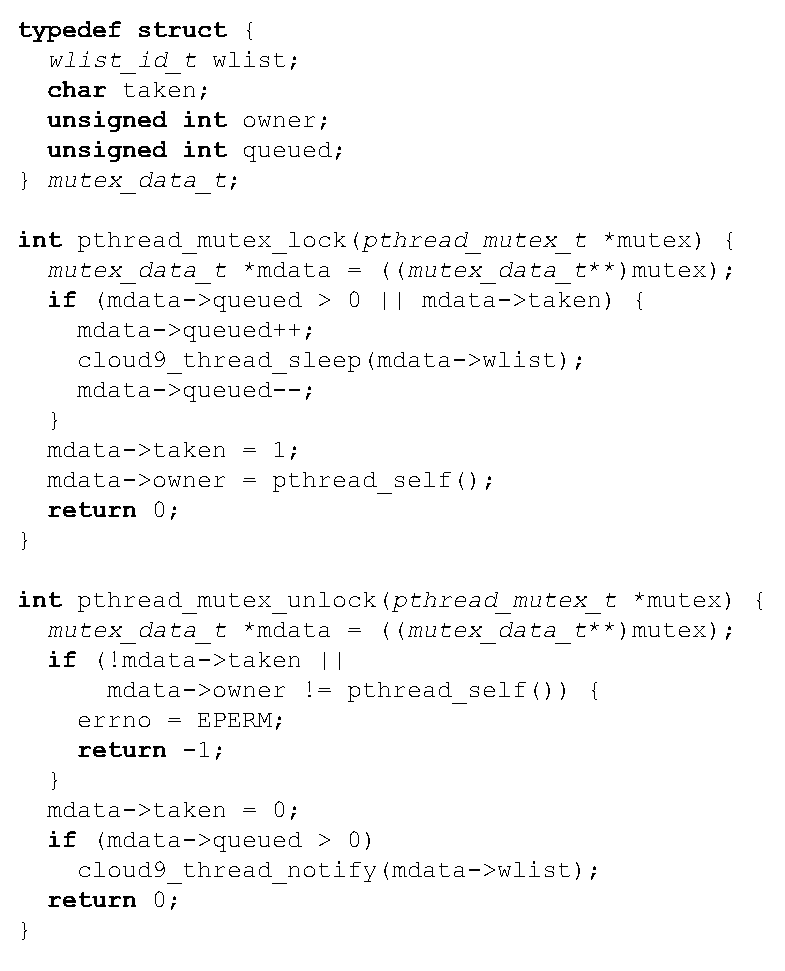
\epsfig{file=figures/cloud9/mutex-model.eps, width=3.2in}
  \caption{Example implementation of pthread mutex operations in \cnine's POSIX environment model.}
  \label{fig:mutexcode}
\end{figure}

\topic{\cnine inherits most of the semantics of the file model from \klee.}  In particular, one can either open a symbolic file (its contents comes from a symbolic block buffer), or a concrete file, in which case a concrete file descriptor is associated with the symbolic one, and all operations on the file are forwarded as external calls on the concrete descriptor. 

\begin{figure}[h!]
  \centering
  \epsfig{file=figures/cloud9/network-model.eps, width=3.0in}
  \caption{A TCP network connection is modeled in \cnine using TX and RX buffers implemented as stream buffers.}
  \label{fig:networkmodel}
\end{figure}

\topic{In addition to file objects, the \cnine POSIX model adds support for networking and pipes.}  Currently, the TCP and UDP protocols are supported over IP and UNIX network types. Since no actual hardware is involved in the packet transmission, we can collapse the entire networking stack into a simple scheme based on two stream buffers (Fig.~\ref{fig:networkmodel}). The network is modeled as a single-IP network with multiple available ports---this configuration is sufficient to connect multiple processes to each other, in order to simulate and test distributed systems. The model also supports pipes through the use of a single stream buffer, similar to sockets.

\topic{The \cnine POSIX model supports polling through the \codebit{select()} interface.}  All the software we tested can be configured to use \codebit{select()}, so it was not necessary to implement other polling mechanisms.  The \codebit{select()} model relies on the event notification support offered by the stream buffers that are used in the implementation of blocking I/O objects (currently sockets and pipes).

\topic{The constraint solver used in \cnine operates on bit vectors; as a result, symbolic formulas refer to contiguous areas of memory.}  In order to reduce the constraint solving overhead, we aim to reduce the amount of intermixing of concrete and symbolic data in the same memory region.  Thus, \cnine's POSIX model segregates concrete from symbolic data by using static arrays for concrete data and linked lists (or other specialized structures) for symbolic data.  We allocate into separate buffers potentially-symbolic data passed by the tested program through the POSIX interface.

\topic{In order to enable testing the systems presented in the evaluation section (Section~\ref{ch:evaluation}), we had to add support for various other components: IPC routines, \codebit{mmap()} calls, time-related functions, etc.}  Even though laborious, this was mostly an engineering exercise, so we do not discuss it further.


%%%%%%%%%%%%%%%%%%%%%%%%%%%%%%%%%%%%%%%%%%%%%%%%%%%%%%%%%%%%%%%%%%%%%%%%%%%%%%%%

\section{Symbolic Test Suites}
\label{sec:cloud9:platform}

Software products and systems typically have large ``hand-made'' test suites; writing and maintaining these suites requires substantial human effort.  \cnine aims to reduce this burden while improving the quality of testing, by offering an easy way to write ``symbolic test suites.'' First, a symbolic test case encompasses many similar concrete test cases into a single symbolic one---each symbolic test a developer writes is equivalent to many concrete ones.  Second, a symbolic test case explores conditions that are hard to produce reliably in a concrete test case, such as the occurrence of faults, concurrency side effects, or network packet reordering, dropping and delay.  Furthermore, symbolic test suites can easily cover unknown corner cases, as well as new, untested functionality.  In this section, we present the API for symbolic tests and illustrate it with a use case.

\subsection{Testing Platform API}

The \cnine symbolic testing API (Tables~\ref{table:globalapi} and~\ref{table:ioctlapi}) allows tests to programmatically control events in the environment of the program under test.  A test suite needs to simply include a \codebit{cloud9.h} header file and make the requisite calls.

\begin{table}[!t]
\addtolength{\tabcolsep}{-2.5pt}
{
\small
\centering
\begin{tabular}{|l|p{50mm}|}
\hline
\textbf{~~~~~Function Name} & \textbf{~~~~~~~~~~~~~~~~~~Description} \\
\hline
\cninesuffix\_make\_symbolic & Mark memory regions as symbolic \\
\hline
\cninesuffix\_fi\_enable & \multirow{2}{4cm}{Enable/disable the injection of faults} \\
\cninesuffix\_fi\_disable & \\
\hline
\cninesuffix\_set\_max\_heap & Set heap size for symbolic \codebit{malloc} \\
\hline
\cninesuffix\_set\_scheduler & Set scheduler policy (e.g., round-robin)\\
\hline
\end{tabular}
\vspace{-4pt}
\caption{\cnine API for setting global behavior parameters.}
\label{table:globalapi}
}
\end{table}

\begin{table}[!t]
\addtolength{\tabcolsep}{-2.5pt}
{
\small
\centering
\begin{tabular}{|l|p{4.8cm}|}
\hline
\textbf{~~Extended Ioctl Code} & \textbf{~~~~~~~~~~~~~~~~Description} \\
\hline
SIO\_SYMBOLIC & Turns this file or socket into a source of symbolic input \\
\hline
SIO\_PKT\_FRAGMENT & Enables packet fragmentation on this socket (must be a stream socket) \\
\hline
SIO\_FAULT\_INJ & Enables fault injection for operations on this descriptor \\
\hline
\end{tabular}
\vspace{-4pt}
\caption{\cnine extended \codebit{ioctl} codes to control environmental events on a per-file-descriptor basis.}
\label{table:ioctlapi}
}
\end{table}

\paragraph{Symbolic Data and Streams} The generality of a test case can be expanded by introducing bytes of symbolic data. This is done by calling \codebit{\cninesuffix\_make\_symbolic}, a wrapper around \codebit{klee\_\allowbreak{}make\_\allowbreak{}symbolic}, with an argument that points to a memory region. \codebit{klee\_make\_symbolic} is a primitive provided by \klee to mark data symbolic.  In addition to wrapping this call, we added several new primitives to the testing API (Table~\ref{table:globalapi}). In \cnine, symbolic data can be written/read to/from files, can be sent/received over the network, and can be passed via pipes. Furthermore, the \codebit{SIO\_SYMBOLIC} \codebit{ioctl} code (Table~\ref{table:ioctlapi}) turns on/off the reception of symbolic bytes from individual files or sockets.

\paragraph{Network Conditions} Delay, reordering, or dropping of packets causes a network data stream to be fragmented.  Fragmentation can be turned on or off at the socket level using one of the \cnine \codebit{ioctl} extensions.  Section~\ref{sec:eval:lighttpd} presents a case where symbolic fragmentation enabled \cnine to prove that a bug fix for the lighttpd web server was incomplete. 

\paragraph{Fault Injection} Calls in a POSIX system can return an error code when they fail. Most programs can tolerate such failed calls, but even high-quality production software misses some~\cite{lfi}. Such error return codes are simulated by \cnine whenever fault injection is turned on. 

\paragraph{Symbolic Scheduler} \cnine provides multiple scheduling policies that can be controlled for purposes of testing on a per-code-region basis.  Currently, \cnine supports a round-robin scheduler and two schedulers specialized for bug finding: a variant of the iterative context bounding scheduling algorithm~\cite{chess} and an exhaustive exploration of all possible scheduling decisions.  


\subsection{Use Case}

Consider a scenario in which we want to test the support for a new \codebit{X-NewExtension} HTTP header, just added to a web server. We show how to write tests for this new feature.

A symbolic test suite typically starts off as an augmentation of an existing test suite; in our scenario, we reuse the existing boilerplate setup code and write a symbolic test case that marks the extension header symbolic. Whenever the code that processes the header data is executed, \cnine forks at all the branches that depend on the header content. Similarly, the request payload can be marked symbolic to test the payload-processing part of the system:

\begin{verbatim}
   char hData[10];
   cloud9_make_symbolic(hData);
   strcat(req, "X-NewExtension: ");
   strcat(req, hData);
\end{verbatim}

The web server may receive HTTP requests fragmented in a number of chunks, returned by individual invocations of the \codebit{read()} system call---the web server should run correctly regardless of the fragmentation pattern.  To test different fragmentation patterns with \cnine, one simply enables symbolic packet fragmentation on the client socket:
\begin{verbatim}
   ioctl(ssock, SIO_PKT_FRAGMENT, RD);
\end{verbatim}

To test how the web server handles failures in the environment, we can ask \cnine to selectively inject faults when the server reads or sends data on a socket by placing in the symbolic test suite calls of the form:
\begin{verbatim}
   ioctl(ssock, SIO_FAULT_INJ, RD | WR);
\end{verbatim}
\cnine can also enable/disable fault injection globally for all file descriptors within a certain region of the code using calls to \codebit{\cninesuffix\_fi\_\allowbreak{}enable} and \codebit{\cninesuffix\_fi\_\allowbreak{}disable}. For simulating low-memory conditions, \cnine provides a \codebit{\cninesuffix\_set\_\allowbreak{}max\_heap} primitive, which can be used to test the web server with different maximum heap sizes.

%%% Local Variables: 
%%% mode: latex
%%% eval: (visual-line-mode)
%%% fill-column: 1000000
%%% TeX-master: "main"
%%% End:


\chapter{Using Language Interpreters as Executable Specifications}
\chaptermark{Interpreters as Executable Specifications}
\label{ch:chef}
\section{Motivation}
\label{sec:supportingintlangs}

\begin{itemize}
  \item Building a symbex engine for high-level languages is hard engineering.
\end{itemize}

Building a correct and complete symbolic execution engine for an interpreted language is generally harder than building one for a low-level language. 
%
Statements of interpreted languages can wrap complex operations that, in lower-level languages, would be implemented through libraries. For instance, Python strings are a built-in type offering more than 30 operations (such as \codebit{find}) as part of the language, implemented natively in the interpreter. 
%
Other language features that allow to inspect or even modify the code itself, i.e., runtime reflection, are even more tedious to implement and very hard to get right.

Finally, besides requiring an enormous initial effort to build a symbolic execution engine that fully supports them, dynamic languages also evolve fast. This implies constant, labor-intensive maintenance and co-evolution of the symbolic execution engine, if it is to keep up with the newest versions of the language.

%%%%%%%%%%%%%%%%%%%%%%%%%%%%%%%%%%%%%%%%%%%%%%%%%%%%%%%%%%%%%%%%%%%%%%%%%%%%%%%%

\section{Symbolically Executing the Interpreter}

\begin{itemize}
\item We can use the interpreter as ``executable language specs'' by plugging it into a low-level (e.g., binary) symbolic execution engine.
\item However, this won't work out of the box.
\end{itemize}

Considering the difficulty of directly supporting interpreted languages, we resort to symbolically executing the interpreter itself, since it completely defines the semantics of the target language as a function of the semantics of the language the interpreter is implemented in.
%
After compiling the interpreter to a format supported by an existing symbolic execution engine, one can symbolically execute an interpreted program by symbolically executing the interpreter with the target program as argument.
%
However, even though in principle this direct approach yields a symbolic execution engine for the target language, it is impractical, due to the engine not being aware of the control flow of the interpreted program.

\paragraph{High- vs. Low-level Program Paths}

\begin{figure}
  \centering
  \includegraphics[width=2.2in]{figures/chef/running-example}
  \caption{Two examples of Python code that lead to path explosion when the interpreter running it is symbolically executed.}
  \label{fig:running-examples}
\end{figure}


An interpreted program conceptually executes both on a high level---the level of the target language---and a low level---the level of the interpreter.
%
A high-level program path is a sequence of values of the high-level program counter (\hlpc). Each \hlpc value corresponds to a program statement or bytecode instruction (both Python and Lua use intermediate bytecode).  Branches can occur explicitly at control flow statements, or implicitly through exceptions.
%
A low-level program path is a sequence of machine instructions from the interpreter binary, including its code for internal bookkeeping (e.g., details of reference counting and garbage collection).

Due to the additional implementation details, a single high-level path can map to multiple low-level paths.
%
Figure~\ref{fig:running-examples} shows two examples of Python code that have few high-level but many low-level paths. The \codebit{validateEmail} method has only two high-level paths, but its use of \codebit{string.find} leads to as many low-level paths as there can be characters in the \codebit{email} string.
%
The second example \codebit{average} may come as more of a surprise: even though it has just a single high-level path, symbolic execution can end up enumerating many low-level paths: Python uses arbitrary-precision integers, so the interpreter may have to iterate over digit vectors of arbitrary length, which can in principle spawn arbitrarily many paths.


\paragraph{Challenges for Search Strategies}
%
The search strategy of a low-level symbolic execution engine is oblivious to the high-level program structure of the target program, and it essentially just tries to cover the interpreter. This generally leads to covering the same high-level paths many times with multiple distinct low-level paths.
%
For instance, a high-level statement like \codebit{find} can lead to hundreds of alternate states, whereas a primitive integer comparison might just create a single one. Therefore, the low-level search strategy is likely to explore multiple ways for \codebit{find} to succeed or fail, without increasing high-level coverage, before eventually exploring the alternate outcome of the comparison.

\begin{figure}
  \centering
  \includegraphics[width=2.8in]{figures/chef/hl-symbex}
  \caption{High-level execution tree (paths A, B, and C), as induced by its low-level execution paths (1--5) for the first running example in Figure~\ref{fig:running-examples}.  Dotted lines segment high-level execution paths into bytecode instructions.  One high-level path may correspond to multiple low-level paths explored.}
  \label{fig:hl-symbex}
\end{figure}

The key is to make the engine aware of the high-level interpreted program. By tracing the values of the \hlpc, the engine can construct a high-level control flow graph~(CFG) on the fly that can be be leveraged by the search strategy.

Alas, a strategy cannot straightforwardly determine future branching points in a high-level CFG: two low-level paths can fork from the same prefix \emph{before} their corresponding high-level paths do.  This can be due to having distinct bytecode instructions for comparisons and conditional jumps, or due to native library calls.  
%
In Figure~\ref{fig:hl-symbex}, three low-level paths fork within the single \hlpc location for \codebit{email.find}. The low-level paths remain on the same high-level path until reaching the branching \hlpc, where they diverge into two distinct high-level paths. The relevant alternate low-level states for covering the distinct high-level paths thus were located away from the location of the code interpreting the high-level control flow statement.
%
The issue of pre-determining branches is present also when exploring regular code, but it is ubiquitous when exploring code on interpreters.



We now present the architecture of \chef (Section~\ref{sec:architecture}) and introduce \cupa, our state selection mechanism (Section~\ref{sec:cupa}). We then describe \cupa optimized for exploring distinct high-level paths (Section~\ref{sec:cupa-paths}) and optimized for high line coverage~(Section~\ref{sec:cupa-coverage}).

\subsection{System Overview}
\label{sec:architecture}

\chef is a platform for language-specific symbolic execution. Provided with an interpreter environment, which acts as an executable language specification, it becomes a symbolic execution engine for the target language (see Figure~\ref{fig:system-arch}).
%
The resulting engine can be used like a hand-written one, in particular for test case generation. When fed with a target program and a symbolic test case (also called test driver or test specification in the literature), it outputs a set of concrete test cases, as shown in Figure~\ref{fig:system-arch}.

\begin{figure}
  \centering
  \includegraphics[width=2.6in]{figures/chef/system-arch}
  \caption{Schema of \chef's architecture.}
  \label{fig:system-arch}
\end{figure}

\chef is built on top of the S2E analysis platform~\cite{s2eSystem}. S2E symbolically executes a virtual machine containing the interpreter and a testing library at the level of machine code,  including the OS kernel, drivers, and user programs.  S2E provides an API that guest code can use to declare memory buffers as symbolic. Comparisons on symbolic values cause S2E to fork new paths, which are enqueued and explored following a search strategy.
%
\chef extends the S2E guest API with a high-level instruction instrumentation call (Section~\ref{sec:exposehlpc}), invoked by interpreters to trace the currently executing high-level path.  The explored high-level paths are used to construct a high-level execution tree and a low-level to high-level mapping (i.e., the data structure shown in Figure~\ref{fig:hl-symbex}).  \chef uses a state selection strategy to maximize the ratio of high-level to low-level paths (Section~\ref{sec:cupa}).

The resulting engine is a correct symbolic execution engine for the target language \textit{as defined by the interpreter}. It is fully precise and theoretically complete, i.e., it will not explore infeasible paths and will eventually explore all paths. The usual limitations of symbolic execution engines apply: completeness holds only under the assumption that the constraint solver can reason about all generated path conditions, and it is understood that exhaustive exploration is usually impossible in finite time.

%%%%%%%%%%%%%%%%%%%%%%%%%%%%%%%%%%%%%%%%%%%%%%%%%%%%%%%%%%%%%%%%%%%%%%%%%%%%%%%%

Consider using symbolic execution for achieving statement coverage on a program containing a function with an input-dependent loop.  At each iteration, the loop forks one additional state (or exponentially many, if there are branches in the loop). A strategy that selects states to explore uniformly is therefore biased toward selecting more states from this function, at the expense of states in other functions that fork less but contribute equally to the statement coverage goal.

We reduce this bias by introducing Class-Uniform Path Analysis (\cupa).
%
The main idea is to group states into classes and then choose uniformly among classes instead of states.  For instance, in the above example, the class of each state could be its current function.  \cupa then first selects uniformly a function, then picks at random a state inside that function.  This way, functions generating many states are still selected with equal probability to others.

In general, \cupa organizes the state queue into a hierarchy of state subsets rooted at the entire state queue (see Figure~\ref{fig:cupa}).  The children of each subset partition the subset according to the \emph{state classification scheme} at their level.  A classification scheme is defined as a function $h: S \rightarrow C$, where $h(s)$ maps each state $s$ into a class value $c$.  States of the same parent with the same class value are sorted into the same child.
%
\begin{figure}
  \centering
  \includegraphics[width=3.2in]{figures/cupa/cupa}
  \caption{\cupa state partitioning.  Each level corresponds to a state classification scheme.  Child nodes partition the parent node according to the classification at their level.}
  \label{fig:cupa}
\end{figure}
%
\cupa selects a new state for exploration by performing a random descent in the classification tree, starting from the root.  When reaching a leaf, the strategy takes out a random state from the state set and returns it to the symbolic execution engine for exploration.  By default, all sibling classes on each level have equal probability of being picked, but they can be assigned weights if required.

A \cupa strategy is parameterized by the number $N$ of levels in the tree and a classification function $h_i$ for each level $i=1 \ldots N$.  \chef uses two instantiations of \cupa: one optimized for covering high-level paths (Section~\ref{sec:cupa-paths}) and one for covering the high-level CFG, i.e., statements (Section~\ref{sec:cupa-coverage}).

%%%%%%%%%%%%%%%%%%%%%%%%%%%%%%%%%%%%%%%%%%%%%%%%%%%%%%%%%%%%%%%%%%%%%%%%%%%%%%%%

\section{Chef Case Study: Path-optimized CUPA}
\label{sec:cupa-paths}

A low-level strategy unaware of the high-level program would be implicitly biased towards picking high-level instructions that fork more low-level states than others, such as string operations or native calls.
%
To mitigate this, we instantiate a two-level \cupa strategy using the following classes:
\begin{enumerate}
\item The location of the state in the high-level symbolic execution tree.  This is the occurrence of the state's high-level program counter (\hlpc) in the unfolded high-level CFG, referred to as the dynamic \hlpc.  We choose the dynamic \hlpc to give each high-level path reaching the \hlpc the same chance to fork and subsequently diverge.
\item The low-level x86 program counter of the state.  This classification reduces the selection bias of ``hot spots'' of path explosion within a single complex instruction, such as a native function call.
\end{enumerate}


%%%%%%%%%%%%%%%%%%%%%%%%%%%%%%%%%%%%%%%%%%%%%%%%%%%%%%%%%%%%%%%%%%%%%%%%%%%%%%%%

\section{Chef Case Study: Coverage-optimized CUPA}
\label{sec:cupa-coverage}

Based on a coverage-optimized strategy introduced by the \klee symbolic execution engine~\cite{klee}, we developed a \cupa instance that partitions states according to their minimum distance to branches leading to uncovered code.
%
Alas, dynamic language interpreters do not generally have a static CFG view of the program, so code that has not been covered yet is not accessible to the search strategy.  The high-level CFG of the target program is dynamically discovered along each execution path.  On this CFG, we employ heuristics that (1) identify the instruction opcodes that may branch, and (2)~weigh the state selection toward states that are closer to these potential branching points.

First, \chef identifies the branching opcodes by collecting all high-level instructions that terminate a basic block with an out-degree in the CFG of at least $2$ (i.e., cause branching in the control flow).   We then eliminate the 10\% least frequent opcodes, which correspond to exceptions or other rare control-flow events.
%
Second, \chef identifies the potential branching points as those instructions in the CFG that have a branching opcode (as previously identified) but currently only one successor.
%
Finally, \chef computes for each execution state the distance in the CFG to the closest such potential branching point.

Having computed this information, we instantiate a two-level \cupa strategy with the following classes:
\begin{enumerate}
\item The static \hlpc of the state in the high-level CFG.  On this level, each class is weighted by $\frac{1}{d}$, where $d$ is the distance in the inferred high-level CFG to the closest potential branching point, making states at locations close to a target more likely to be selected.
\item The state itself (so each partition has a single element).  On this level, the states are weighted by their \textit{fork weight}.
\end{enumerate}

Fork weight is computed by counting the number of consecutive forks at the same low-level program counter (i.e., at an input-dependent loop in machine code).  States $1, \ldots, n$ forking from the same path at the same location get weights $p^n, p^{n-1}, \ldots, 1$, where $p < 1$ de-emphasizes states forked earlier ($p = 0.75$ in our implementation).  The last state to fork at a certain location thus gets maximum weight, because alternating the last decision in a loop is often the quickest way to reach different program behavior (e.g., to satisfy a string equality check).

%%%%%%%%%%%%%%%%%%%%%%%%%%%%%%%%%%%%%%%%%%%%%%%%%%%%%%%%%%%%%%%%%%%%%%%%%%%%%%%%

\section{High-level Symbolic Execution}
\begin{itemize}
\item Define the concept of high-level path.
\item Define the notion of high-level state.  Introduce the notion of completeness model, and discuss the tradeoffs between each.
\end{itemize}

%%%%%%%%%%%%%%%%%%%%%%%%%%%%%%%%%%%%%%%%%%%%%%%%%%%%%%%%%%%%%%%%%%%%%%%%%%%%%%%%

\section{High-level Control Flow Reconstruction}
\begin{itemize}
\item We need to bridge the gap between the stream of x86 instructions and stream of high-level instructions.
\item Manual approach: interpreter loop annotation.
\item Automated approach: use calibration program + look for memory access patterns inside the interpreter.
\end{itemize}

We now explain how to prepare an interpreter for \chef: the first and mandatory step is to instrument the main interpreter loop to report \hlpcs (Section~\ref{sec:exposehlpc}); the second and optional step is to optimize the interpreter for efficient symbolic execution (Section~\ref{sec:optimzeforsymbex}).  \chef provides an API (Table~\ref{tab:api}) that will be explained along with its use.  Finally, we discuss the remaining work of building a language-specific testing API to the resulting engine (Section~\ref{sec:testingAPI}).

\begin{table}
\centering
\small
\begin{tabular}{| l | l | }
\hline
\textbf{API Call} & \textbf{Description} \\
\hline
\codebit{log\_pc(pc, opcode)} & Log the interpreter PC and opcode \\
\hline
\codebit{start\_symbolic()} & Start the symbolic execution \\
\codebit{end\_symbolic()} & Terminate the symbolic state \\
\hline
\codebit{make\_symbolic(buf)} & Make buffer symbolic \\
\codebit{concretize(buf)} & Concretize buffer of bytes \\
\codebit{upper\_bound(value)} & Get maximum value for expression\\
                              & on current path \\
\codebit{is\_symbolic(buf)} & Check if buffer is symbolic \\
\codebit{assume(expr)} & Assume constraint \\
\hline
\end{tabular}
\caption{The \chef API used by the interpreters running inside the S2E VM.}
\label{tab:api}
\end{table}

To reconstruct the high-level program paths and CFG, \chef needs to identify the high-level instructions executed on each low-level path.  \chef provides the \codebit{log\_pc(pc, opcode)} API call to the interpreter, which declares the current high-level program location and the type (opcode) of the next instruction.  A high-level instruction is executed in between two consecutive \codebit{log\_pc} calls.
%
Interpreters typically contain a main interpretation loop that \codebit{switch}-es over the type of the current instruction and invokes specific handlers.  The \codebit{log\_pc} call can be added conveniently at the head of the interpreter loop.

In our design, we make minimal assumptions about the language structure, so the \hlpc and opcode values are opaque; the \cupa strategies were designed accordingly.  Nonetheless, more specific versions of the system could add structure to the two values, e.g. provide a pair of function name and offset as \hlpc.  The additional information can be used by \chef to improve the exploration heuristics (e.g., by creating a \cupa class).

The granularity of \codebit{log\_pc} calls depends on the language structure.  \chef's correctness does not depend on the specific instrumentation pattern, but the more closely the reported \hlpc corresponds to statements in the target program, the more accurately \cupa can cluster states. In the extreme, if \codebit{log\_pc} is never invoked, \chef would see the entire program as a single high-level instruction and lose the advantage of \cupa clustering for \hlpcs.

%%%%%%%%%%%%%%%%%%%%%%%%%%%%%%%%%%%%%%%%%%%%%%%%%%%%%%%%%%%%%%%%%%%%%%%%%%%%%%%%

\section{Interpreter Optimizations}
\label{sec:optimzeforsymbex}

\begin{itemize}
\item Goal: reduce path explosion in the interpreter.
\item Approach: ``anti-optimizations'' that slow down linear execution, but boost multi-path execution.
\item Hash neutralization.
\item String interning.
\item Handling memory allocations.
\end{itemize}

In order to maximize performance, interpreters make heavy use of special cases and sophisticated data structures.  Unfortunately, these features hurt the performance of symbolic execution by amplifying path explosion and increasing the complexity of symbolic formulas~\cite{overify}.

We identify a number of easy optimizations that preserve the interpretation semantics but significantly improve symbolic execution performance.  The optimizations use the \chef API in the last block of rows in Table~\ref{tab:api}.

\paragraph{Neutralizing Hash Functions}

Hash functions are especially common in interpreters, due to the internal use of hash tables for associative data structures (e.g., Python dictionaries or Lua tables).  However, they are generally a problem in symbolic execution: a symbolic value added to a hash table (a)~creates constraints that essentially ask the constraint solver to reverse a hash function, which is often hard, and (b)~causes the exploration to fork on each possible hash bucket the value could fall into.
%
A simple and effective optimization is to \emph{neutralize the hash function}, i.e., replace it with a degenerate one returning a single constant. This change honors the usual contracts for hash functions (equal objects have equal hashes) and will turn hash lookups into list traversals.

\paragraph{Avoiding Symbolic Pointers}

Input-dependent pointers (also referred to as symbolic pointers) may point to multiple locations in the program memory, so a pointer dereference operation would have to be resolved for each possible location.  In practice, symbolic execution engines deal with this situation in one of two ways:
%
(a)~fork the execution state for each possible concrete value the symbolic pointer can take; or
%
(b)~represent the dereference symbolically as a read operation from memory at a symbolic offset and let the constraint solver ``deal'' with it.
%
Both ways hurt symbolic execution, either by causing excessive path explosion or by burdening the constraint solver.

While there is no generic way to avoid symbolic pointers other than concretizing their values (the \codebit{concretize} API call) at the price of losing completeness, there are specific cases where they can be avoided.

First, \emph{the size of a buffer can be concretized} before allocation.  A symbolic size would most likely cause a symbolic pointer to be returned, since a memory allocator computes the location of a new block based on the requested size.  To avoid losing completeness, a symbolic execution-aware memory allocator can determine a (concrete) upper bound on the requested size and use that value for reserving space, while leaving the original size variable symbolic.  This way, memory accesses to the allocated block would not risk being out of bounds.  Figure~\ref{fig:sym-malloc} shows how the \chef API is used to wrap a call to the \codebit{malloc} function in the standard C library.

\begin{figure}
  \centering
  \includegraphics[width=2.6in]{figures/chef/mallocopt}
  \caption{Example of a symbolic execution-aware \codebit{malloc} function wrapper created using the \chef API.  If the allocation size is symbolic, the wrapper determines its upper bound and issues a concrete request to the underlying implementation.}
  \label{fig:sym-malloc}
\end{figure}

Second, \emph{caching and ``interning'' can be eliminated}.  Caching computed results and value interning (i.e., ensuring that a single copy of each possible value of a type is created) are common ways to improve the performance of interpreters.  Alas, when a particular value is computed, its location in memory becomes dependent on its value. If the value was already in the cache or in the interned store, it is returned from there, otherwise a new value is computed.  During symbolic execution, this logic becomes embedded in the value of the returned pointer, which becomes symbolic.  Disabling caching and interning may hurt the native performance of the program, but it can give a significant boost when running inside a symbolic execution engine.

\paragraph{Avoiding Fast Paths}

A common way to speed-up the native performance of a function is to handle different classes of inputs using faster specialized implementations (``fast paths'').  For example, a string comparison automatically returns false if the two strings have different lengths, without resorting to byte-wise comparison.

Fast paths may hurt symbolic execution because they cause symbolic branches in the code checking for the special input conditions.  \emph{Eliminating short-circuited returns} can reduce path explosion.  Instead of returning to the caller as soon as it produced an answer, the function continues running and stops on an input-independent condition.  For example, when comparing two strings of concrete length, a byte-wise string comparison would then traverse the entire string buffers in a single execution path, instead of returning after the first difference found.


\subsection{Testing API}
\label{sec:testingAPI}

Programs to be tested can be fed symbolic inputs by marking input buffers with \codebit{make\_symbolic} and defining conditions over the input with the \codebit{assume} call, in accordance to the test specification.  Note that the buffer is a memory region of concrete bounds.  It is the job of the symbolic test library in the interpreter VM to convert from the language data structures (e.g., strings, integers) to the memory locations used to store the data in the interpreter implementation.

%%% Local Variables: 
%%% mode: latex
%%% eval: (visual-line-mode)
%%% fill-column: 1000000
%%% TeX-master: "main"
%%% End:


\chapter{Class-Uniform Path Analysis}
\label{ch:cupa}
\section{Overview}

\begin{itemize}
\item Rationale: Path explosion is clustered in fork bombs.
\item Idea: Isolate the fork bombs into groups selected uniformly for execution.  The intuition is that this will increase state diversity and hence increase the overall exploration throughput.
\item CUPA classes can be nested.
\end{itemize}

%%%%%%%%%%%%%%%%%%%%%%%%%%%%%%%%%%%%%%%%%%%%%%%%%%%%%%%%%%%%%%%%%%%%%%%%%%%%%%%%

\section{Chef Case Study: Path-optimized CUPA}

%%%%%%%%%%%%%%%%%%%%%%%%%%%%%%%%%%%%%%%%%%%%%%%%%%%%%%%%%%%%%%%%%%%%%%%%%%%%%%%%

\section{Chef Case Study: Coverage-optimized CUPA}

%%% Local Variables: 
%%% mode: latex
%%% eval: (visual-line-mode)
%%% fill-column: 1000000
%%% TeX-master: "main"
%%% End:



\chapter{Parallel Symbolic Execution}
\label{ch:parsymbex}
\section{Motivation}

\begin{itemize}
\item ``Throw hardware at the problem''.
\item No linear scalability demonstrated with previous approaches. Main cause: imbalanced tree shape, unknown a priori.
\item Foundation for a software testing service.
\end{itemize}

%%%%%%%%%%%%%%%%%%%%%%%%%%%%%%%%%%%%%%%%%%%%%%%%%%%%%%%%%%%%%%%%%%%%%%%%%%%%%%%%

\section{Overview}

\begin{itemize}
\item Introduce workers + load balancer.
\item Goal: disjoint and complete tree exploration.
\item Each worker explores tree independently, with minimal synchronization overhead.
\end{itemize}

%%%%%%%%%%%%%%%%%%%%%%%%%%%%%%%%%%%%%%%%%%%%%%%%%%%%%%%%%%%%%%%%%%%%%%%%%%%%%%%%

\section{Worker-level Operation}

\begin{itemize}
\item Introduce dead, fence, and candidate nodes.
\end{itemize}

%%%%%%%%%%%%%%%%%%%%%%%%%%%%%%%%%%%%%%%%%%%%%%%%%%%%%%%%%%%%%%%%%%%%%%%%%%%%%%%%

\section{Cluster-level Operation}

\begin{itemize}
\item Describe the load balancer operation.
\end{itemize}

%%% Local Variables: 
%%% mode: latex
%%% eval: (visual-line-mode)
%%% fill-column: 1000000
%%% TeX-master: "main"
%%% End:



\chapter{Evaluation}
\label{ch:evaluation}
\section{Prototypes}

\subsection{Cloud9}

We developed a \cnine prototype on top of the \klee~\cite{klee} symbolic execution engine.  The prototype has 7 \kloc.
%
The \klee modifications to support the symbolic OS abstractions amount to roughly 2 \kloc, while the rest consists of the POSIX model built on top of the abstractions.

\subsection{Chef}

We used \chef to generate symbolic execution engines for Python~(\S\ref{sec:python}) and Lua~(\S\ref{sec:lua}). Table~\ref{tab:pychanges} summarizes the effort to set up the two interpreters for \chef.  The necessary changes to the interpreter amount to 321 lines of code for Python and 277 for Lua.
%
The total developer time was 5 person-days for Python and 3 person-days for Lua, which is orders of magnitude smaller than the effort required for building a complete symbolic execution engine from scratch.  

\begin{table}
\centering
\small
\begin{tabular}{|@{\hspace*{4pt}}l@{\hspace*{4pt}}|@{\hspace*{4pt}}r@{\hspace*{4pt}}|@{\hspace*{4pt}}r@{\hspace*{4pt}}|}
\hline
\textbf{Component} & \textbf{Python} & \textbf{Lua}\\
\hline
Interpreter core size (C LoC) & 427,435 & 14,553 \\
\hline
\hline
HLPC instrumentation (C LoC) & 47 (0.01\%) & 44 (0.30\%) \\
Sym. optimizations (C LoC) & 274 (0.06\%) & 233 (1.58\%) \\
\hline
Native extensions (C LoC) & 1,320 (0.31\%) & 154 (1.06\%) \\
Test library (Python/Lua LoC) & 103 & 87 \\
\hline
\hline
Developer time (person-days) & 5 & 3 \\
\hline
\end{tabular}
\caption{Summary of the effort required to support Python and Lua in \chef.  The first row is the interpreter size without the standard language library. The next two rows are changes in the interpreter core, while the following two constitute the symbolic test library.  The last item indicates total developer effort.}
\label{tab:pychanges}
\end{table}

\subsubsection{Symbolic Execution Engine for Python}
\label{sec:python}

\paragraph{Interpreter Instrumentation}

We instrumented the CPython interpreter 2.7.3 for use with \chef, according to the guidelines presented in~\S\ref{sec:recipe}.

Python programs are composed of modules, corresponding to Python source files.  Each source file is compiled into an interpreter-specific bytecode format, i.e., each source statement is translated into one or more lower-level primitive instructions.  The instructions are grouped into blocks, corresponding to a single loop nesting, function, method, class, or global module definition.
%
We define an \hlpc as the concatenation of the unique block address of the top frame on the stack and the current instruction offset inside the block. We instrumented the Python interpreter to pass this program location to \chef; this required adding less than 50 LoC to the main interpreter loop.

We performed several optimizations on the Python interpreter: we neutralized the hash functions of strings and integers, which are the most common objects; we concretized the memory sizes passed to the garbage-collected memory allocator; and we eliminated interning for small integers and strings.    
%
Most optimizations involved only adding preprocessor directives for conditional compilation of blocks of code.
%
We gathered the optimizations under a new \codebit{--with-symbex} flag of the interpreter's \codebit{./configure} script.

\paragraph{Symbolic Tests}

To validate the usefulness of the resulting symbolic execution engine, we use it as a test case generation tool.  To this end, we implemented a symbolic test library as a separate Python package, used both inside the guest virtual machine, and outside, during test replay.
%
Figure~\ref{fig:sample-test} is an example of a symbolic test class for the \codebit{argparse} command-line interface generator. It sets up a total of 12 symbolic characters of input: two 3-character symbolic arguments to configure the command-line parser plus another two to exercise the parsing functionality.

The test class derives from the library's \codebit{SymbolicTest} class, which provides two methods to be overridden: \codebit{setUp}, which is run once before the symbolic test starts, and \codebit{runTest}, which creates the symbolic input and can check properties.  The symbolic inputs are created by calling the \codebit{getString} and \codebit{getInt} methods in the \codebit{SymbolicTest} API.

\begin{figure}
  \centering
  \includegraphics[width=3.2in]{figures/evaluation/symtest}
  \caption{The symbolic test used to exercise the functionality of the Python \codebit{argparse} package.}
  \label{fig:sample-test}
\end{figure}

A symbolic test is executed by a symbolic test runner, which is also part of the library.  The runner can work in either symbolic or replay mode. 
%
In \emph{symbolic mode}, the runner executes inside the guest virtual machine.  It creates a single instance of the test class, whose \codebit{getString} and \codebit{getInt} methods create corresponding Python objects and invoke the \codebit{make\_symbolic} call to mark their memory buffers as symbolic.
%
In \emph{replay mode}, the runner creates one instance of the test class for each test case created by \chef. The \codebit{getString} and \codebit{getInt} methods return the concrete input assignment of the test case.


\subsubsection{Symbolic Execution Engine for Lua}
\label{sec:lua}

Lua is a lightweight scripting language mainly used as an interpreter library to add scripting capabilities to software written in other languages. However, it also has a standalone interpreter and several Lua-only projects exist. We generated a symbolic execution engine for Lua based on version 5.2.2 of the Lua interpreter.

\paragraph{Interpreter Instrumentation}

Similar to Python, Lua programs are composed of one or more Lua source files, compiled into a bytecode format.  The code is compiled into a set of functions that operate on a global stack of values.  Each function is composed of a sequence of bytecode instructions, where each instruction is defined by an offset, opcode, and parameters.
%
We construct the \hlpc as the concatenation of the unique address of the function in the top frame and the current instruction offset being executed.  The instrumentation amounts to less than 50 LoC added to the interpreter loop.

We optimized the Lua interpreter for symbolic execution by eliminating string interning.  In addition, we configured the interpreter to use integer numbers instead of the default floating point, for which S2E does not support symbolic expressions.  This change was easy, because it was available as a macro definition in the interpreter's configuration header.

%%%%%%%%%%%%%%%%%%%%%%%%%%%%%%%%%%%%%%%%%%%%%%%%%%%%%%%%%%%%%%%%%%%%%%%%%%%%%%%%

\section{Experimental Setup and Testing Targets}

\subsection{Running Low-level Systems with Cloud9}



\subsection{Targeting Python and Lua Packages with Chef}

All reported \chef experiments were performed on a 48-core 2.3 GHz AMD Opteron 6176 machine with 512 GB of RAM, running Ubuntu 12.04. Each \chef invocation ran on 1 CPU core and used up to 8 GB of RAM on average.

\paragraph{Testing Targets}

\begin{table*}[!ht]
\centering
\footnotesize
\begin{tabular}{@{\hspace*{5pt}}l@{\hspace*{11pt}}r@{\hspace*{11pt}}l@{\hspace*{11pt}}l|r|c|c@{\hspace*{5pt}}}
\textbf{Package} & \textbf{LOC} & \textbf{Type} & \textbf{Description} & \textbf{Coverable LOC} & \textbf{Exceptions} & \textbf{Hangs}\\
\hline
\rule{0pt}{12pt}\textbf{Python} & & & & & \\
argparse$^{*}$ & 1,466 & System & Command-line interface & 1,174 & 4 / 0 & --- \\
ConfigParser$^{*}$ & 451 & System & Configuration file parser & 145 & 1 / 0 & --- \\
%
HTMLParser$^{*}$ & 623 & Web & HTML parser & 582 & 1 / 0 & --- \\
simplejson 3.10 & 1,087 & Web & JSON format parser & 315 & 2 / 0 & --- \\
%% webapp2 2.5.2 & 1,986 & Web & Web framework & & \\
%
unicodecsv 0.9.4 & 126 & Office & CSV file parser & 95 & 1 / 0 & --- \\
xlrd 0.9.2 & 7,241 & Office & Microsoft Excel reader & 4,914 & 5 / 4 & --- \\[2pt]
%
\hline
\rule{0pt}{12pt}\textbf{Lua} & & & & & & \\
cliargs 2.1-2 & 370 & System & Command-line interface & 273 & --- & --- \\
haml 0.2.0-1 & 984 & Web & HTML description markup & 775 & --- & --- \\
sb-JSON v2007 & 454 & Web & JSON format parser & 329 & --- & $\checkmark$ \\
markdown 0.32 & 1,057 & Web & Text-to-HTML conversion & 673 & --- & --- \\
moonscript 0.2.4-1 & 4,634 & System & Language that compiles to Lua & 3,577 & --- & --- \\[2pt]
%
\hline
\rule{0pt}{12pt}\textbf{TOTAL} & 18,493 & & & 12,852 & & \\
\end{tabular}
\caption{Summary of testing results for the Python and Lua packages
  used for evaluation. Items with (*) represent standard library
  packages.
  Exception numbers indicate total / undocumented exception types
  discovered.}
\label{tab:targets}
\end{table*}

We evaluated the symbolic execution engines for Python and Lua on 6 Python and 5 Lua packages, respectively, including system, web, and office libraries. In total, the tested code in these packages amounts to about $12.8$ KLOC.  We chose the latest versions of widely used packages from the Python standard library, the Python Package Index, and the Luarocks repository.  Whenever possible, we chose the pure interpreted implementation of the package over the native optimized one (e.g., the Python \codebit{simplejson} package). The first five columns of Table~\ref{tab:targets} summarize the package characteristics; LOC numbers were obtained with the \codebit{cloc} tool~\cite{cloc}.

The reported package sizes exclude libraries, native extension modules, and the packages' own test suites.
However, the packages ran in their unmodified form, using all the language features and libraries they were designed to use, including classes, built-in data structures (strings, lists, dictionaries), regular expressions, native extension modules, and reflection.  

All testing targets have a significant amount of their functionality written in the interpreted language itself; we avoided targets that are just simple wrappers around native extension modules (written in C or C++) in order to focus on the effectiveness of \chef at distilling high-level paths from low-level symbolic execution.  Nevertheless, we also included libraries that depend on native extension modules.  For instance, all the testing targets containing a lexing and parsing component use Python's standard regular expression library, which is implemented in C.
% The execution of parsers heavily depends on possible regular expression matches on input strings.
To thoroughly test these parsers, it is important to also symbolically execute the native regular expression library. For this, the binary symbolic execution capabilities of \chef are essential.

\paragraph{Methodology: Symbolic Tests}

For each package, we wrote a symbolic test that invokes the package's entry points with one or more symbolic strings.  
%The symbolic tests invoke the code under test in a generic manner without specific checks.  
Figure~\ref{fig:sample-test} in \S\ref{sec:symbolictests} is an example of such a symbolic test.

Each symbolic test ran for 30 minutes within \chef, after which we replayed the collected high-level tests on the host machine, in a vanilla Python/Lua environment, to confirm test results and measure line coverage.  To compensate for the randomness in the state selection strategies, we repeated each experiment 15 times.  In each graph we present average values and error margins as +/- one standard deviation.

For our experiments, we did not use explicit specifications, but relied on generic checks for finding common programming mistakes.  For both Python and Lua, we checked for interpreter crashes and potential hangs (infinite loops). 
For Python---which, unlike Lua, has an exception mechanism---we also flagged whenever a test case led to unspecified exceptions being thrown.
%
In general, one could find application-specific types of bugs by adding specifications in the form of assertions, as in normal unit tests.

\paragraph{Methodology: Coverage Measurement}

Line or statement coverage remains widely used, even though its meaningfulness as a metric for test quality is disputed. We measure and report line coverage to give a sense of what users can expect from a test suite generated fully automatically by a symbolic execution engine based on \chef.  For Python, we rely on the popular \codebit{coverage} package, and for Lua we use the \codebit{luacov} package.

Since our prototype only supports strings and integers as symbolic program inputs, we count only the lines of code that can be reached using such inputs. We report this number as ``coverable LOC'' in the fifth column of Table~\ref{tab:targets}, and use it in our experiments as a baseline for what such a symbolic execution engine could theoretically cover directly.  For example, for the \codebit{simplejson} library, this includes only code that decodes JSON-encoded strings, not code that takes a JSON object and encodes it into a string. Note that, in principle, such code could still be tested and covered by writing a more elaborate symbolic test that sets up a JSON object based on symbolic primitives~\cite{paas-testing}.

%%%%%%%%%%%%%%%%%%%%%%%%%%%%%%%%%%%%%%%%%%%%%%%%%%%%%%%%%%%%%%%%%%%%%%%%%%%%%%%%

\section{Test Suite Generation Effectiveness}

%%%%%%%%%%%%%%%%%%%%%%%%%%%%%%%%%%%%%%%%%%%%%%%%%%%%%%%%%%%%%%%%%%%%%%%%%%%%%%%%

\section{Bug Finding Effectiveness}

%%%%%%%%%%%%%%%%%%%%%%%%%%%%%%%%%%%%%%%%%%%%%%%%%%%%%%%%%%%%%%%%%%%%%%%%%%%%%%%%

\section{Scalability Analysis}

Discuss scalability of the Cloud9 parallelization algorithm.

Discuss overhead of Chef compared to hand-written engines.

%%% Local Variables: 
%%% mode: latex
%%% eval: (visual-line-mode)
%%% fill-column: 1000000
%%% TeX-master: "main"
%%% End:


\chapter{Towards a Cloud Testing Service for PaaS}
\label{ch:paas}
\section{Motivation}

\begin{itemize}
\item ``Throw hardware at the problem''.
\item No linear scalability demonstrated with previous approaches. Main cause: imbalanced tree shape, unknown a priori.
\item Foundation for a software testing service.
\end{itemize}

Testing a program consists of exercising many different paths through it and checking whether they ``do the right thing.''  In other words, testing is a way to produce partial evidence of correctness, and thus increase confidence in the tested software.  Yet, due to the typically poor coverage one can get today, testing often turns into a mere hunt for bugs.

In practice, most software test harnesses consist of manually written tests that are run periodically; regression test suites provide an automated way of checking whether new bugs have entered the code~\cite{codeComplete}.  Such suites tend to be tedious to write and maintain but, once in place, they can be reused and extended.  In practice, the state of the art consists mostly of fuzzing, i.e., trying various inputs in the hope of finding bugs and improving test coverage.

In research, the state of the art consists of model checkers and automated test generators based on symbolic execution~\cite{dart,klee}.  Instead of running a program with regular concrete inputs (e.g., $x\!=\!5$), symbolic execution consists of running a program with ``symbolic'' inputs that can take on all values allowed by the type (e.g., $x\!=\!\lambda$, where $\lambda \in \mathbb{N}$).  Whenever a conditional branch is encountered that involves a predicate $\pi$ that depends (directly or indirectly) on $x$, state and execution are forked into two alternatives: one following the then-branch ($\pi$) and another following the else-branch ($\neg \pi$). The two executions can now be pursued independently.  When a bug is found, test generators can compute concrete values for program inputs that take the program to the bug location.  This approach is efficient because it analyzes code for entire classes of inputs at a time, thus avoiding the redundancy inherent in fuzzing.

The {\em first challenge} for such tools is path explosion, as mentioned earlier.  One way to cope is to memoize the symbolic execution of sub-paths into test summaries that can be subsequently reused when the same sub-path is encountered again, as done in compositional test generation~\cite{godefroid:compdyntest}.  Alternatively, it is possible to use various heuristics to prioritize the most interesting paths first, as done in \klee~\cite{klee}.  Another approach is to execute symbolically only paths that are of interest to the test, as done in selective symbolic execution~\cite{s2e}.

We pursue a complementary approach---{\em parallel symbolic execution}---in which we symbolically execute a program in parallel on a cluster, thus harnessing the machines into a ``distributed computer'' whose aggregate CPU and memory surpass that of an individual machine.  An alternative to a cluster-based approach would be to run a classic single-node symbolic execution engine on a Blue Gene-like supercomputer with vast shared memory and CPUs communicating over MPI.  Supercomputers, however, are expensive, so we favor instead clusters of cheap commodity hardware.  

One way to parallelize symbolic execution is by statically dividing up the task among nodes and having them run independently.   However, when running on large programs, this approach leads to high workload imbalance among nodes, making the entire cluster proceed at the pace of the slowest node~\cite{parallelSymbex}.  If this node gets stuck, for instance, while symbolically executing a loop, the testing process may never terminate.  Parallelizing symbolic execution on shared-nothing clusters in a way that scales well is difficult.

The {\em second challenge} is mediating between a program and its environment, i.e., symbolically executing a program that calls into libraries and the OS, or communicates with other systems, neither of which execute symbolically.  One possible approach is to simply allow the call to go through into the ``concrete'' environment (e.g., to write a file)~\cite{dart,exe}; unfortunately, this causes the environment to be altered for \emph{all} forked executions being explored in parallel, thus introducing inconsistency.  Another approach is to replace the real environment with a symbolic model, i.e., a piece of code linked with the target program that provides the illusion of interacting with a symbolically executing environment.  For instance, \klee uses a symbolic model of the file system~\cite{klee}. Of course, real-world programs typically interact in richer ways than just file I/O: they fork processes, synchronize threads, etc.  

We originally viewed the building of a complete environment model as an engineering task, but our ``mere engineering'' attempt failed: for any functionality that, in a normal execution, requires hardware support (such as enforcing isolation between address spaces), the core symbolic execution engine had to be modified.  The research challenge therefore is to find the minimal set of engine primitives required to support a rich model of a program's environment. 

The {\em third challenge} is using an automated test generator in the context of a development organization's quality assurance processes.  To take full advantage of the automated exploration of paths, a testing tool must provide ways to control all aspects of the environment.  For example, there needs to be a clean API for injecting failures at the boundary between programs and their environment, there must be a way to control thread schedules, and so on.  There should be a way to programmatically orchestrate all environment-related events, but doing so should not require deep expertise in the technology behind the testing tools themselves.

The work presented here aims to address these three challenges.  Cluster-based parallel symbolic execution (Section~\ref{ch:parsymbex}) provides the illusion of running a classic symbolic execution engine on top of a large, powerful computer.  Without changing the exponential nature of the problem, parallel symbolic execution harnesses cluster resources to make it feasible to run automated testing on larger systems than what was possible until now. Our work complements and benefits all tools and approaches based on symbolic execution.  We describe a way to accurately model the environment (Section~\ref{ch:cloud9}) with sufficient completeness to test complex, real software, like the Apache web server and the Python interpreter.  We present the APIs and primitives that we found necessary in developing a true testing platform (Section~\ref{sec:platform}).  We show how using these APIs enables, for instance, finding errors in bug patches by reproducing environment conditions which otherwise would have been hard or impossible to set up with regular test cases.

In this section we present the design of the \cnine engine, focusing on the algorithmic aspects: after a conceptual overview (Section~\ref{sec:concept}), we describe how \cnine operates at the worker level (Section~\ref{sec:workerView}) and then at the cluster level (Section~\ref{sec:loadBalancing}).

%%%%%%%%%%%%%%%%%%%%%%%%%%%%%%%%%%%%%%%%%%%%%%%%%%%%%%%%%%%%%%%%%%%%%%%%%%%%%%%%

\section{Overview}
\label{sec:concept}

\begin{itemize}
\item Introduce workers + load balancer.
\item Goal: disjoint and complete tree exploration.
\item Each worker explores tree independently, with minimal synchronization overhead.
\end{itemize}

%--------------------------------------------------
\paragraph{Classic Symbolic Execution}

\cnine employs symbolic execution, an automated testing technique that has recently shown a lot of
promise~\cite{dart,klee}. 

A symbolic execution engine (SEE) executes a program with unconstrained symbolic inputs.  When a branch involves symbolic values, execution forks into two parallel executions (see Section~\ref{sec:overview}), each with a corresponding clone of the program state.  Symbolic values in the clones are {\em constrained} to make the branch condition evaluate to false (e.g., $\lambda\!\ge${\small MAX}) respectively true (e.g., $\lambda\!<${\small MAX}). Execution recursively splits into sub-executions at each subsequent branch, turning an otherwise linear execution into an {\em execution tree} (Fig.~\ref{fig:exectree}). 

\begin{figure}[h!]
  \centering
  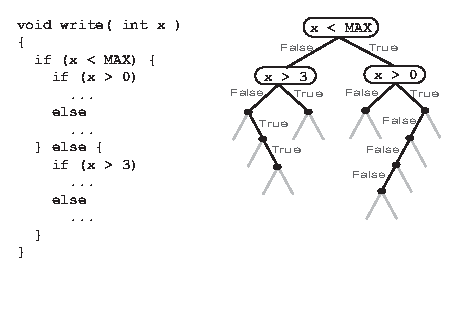
\epsfig{file=figures/parsymbex/execTree.eps, width=2.7in}
  \vspace{-10mm}
  \caption{Symbolic execution produces an execution tree.}
  \label{fig:exectree}
  \vspace{-2mm}
\end{figure}

In this way, all execution paths in the program are explored.  To ensure that only feasible paths are explored, the SEE uses a constraint solver to check the satisfiability of each branch's predicate, and it only follows satisfiable branches.  If a bug is encountered (e.g., a crash or a hang) along one of the paths, the solution to the constraints accumulated along that path yields the inputs that take the tested program to the bug---these inputs constitute a {\em test case}.

%--------------------------------------------------
\paragraph{Parallel Symbolic Execution}

Since the size of the execution tree is exponential in the number of branches, and the complexity of constraints increases as the tree deepens, state-of-the-art SEEs can quickly bottleneck on CPU and memory even for programs with just a couple \kloc.  We therefore build a parallel SEE that runs on a commodity cluster and enables ``throwing hardware at the problem.''

The key design goal is to enable individual cluster nodes to explore the execution tree independently of each other.  One way of doing this is to statically split the execution tree and farm off subtrees to worker nodes.  Alas, the contents and shape of the execution tree are not known until the tree is actually explored, and finding a balanced partition (i.e., one that will keep all workers busy) of an unexpanded execution tree is undecidable.  Besides subtree size, the amount of  memory and CPU required to explore a subtree is also undecidable, yet must be taken into account when partitioning the tree. Since the methods used so far in parallel model checkers~\cite{swarm,spin:multicore-modelchecking} rely on static partitioning of a finite state space, they cannot be directly applied to the present problem. Instead, \cnine partitions the execution tree {\em dynamically}, as the tree is being explored. 

%--------------------------------------------------
\paragraph{Dynamic Distributed Exploration}

\cnine consists of wor\-ker nodes and a load balancer (LB).  Workers run independent SEEs, based on \klee~\cite{klee}.  They explore portions of the execution tree and send statistics on their progress to the LB, which in turn instructs, whenever necessary, pairs of workers to balance each other's work load.  Encoding and transfer of work is handled directly between workers, thus taking the load balancer off the critical path.

The goal is to dynamically partition the execution tree such that the parts are {\em disjoint} (to avoid redundant work) and together they {\em cover} the global execution tree (for exploration to be complete).  We aim to minimize the number of work transfers and associated communication overhead.  A fortuitous side effect of dynamic partitioning is the transparent handling of fluctuations in resource quality, availability, and cost, which are inherent to large clusters in cloud settings.

\cnine operates roughly as follows: The first component to come up is the load balancer.  When the first worker node $W_1$ joins the \cnine cluster, it connects to the LB and receives a ``seed'' job to explore the entire execution tree.  When the second worker $W_2$ joins and contacts the LB, it is instructed to balance $W_1$'s load, which causes $W_1$ to break off some of its unexplored subtrees and send them to $W_2$ in the form of {\em jobs}.  As new workers join, the LB has them balance the load of existing workers.  The workers regularly send to the LB status updates on their load in terms of exploration jobs, along with current progress in terms of code coverage, encoded as a bit vector.  Based on workers' load, the LB can issue job transfer requests to pairs of workers in the form $\langle$~source worker, destination worker, \# of jobs~$\rangle$.  The source node decides which particular jobs to transfer.

%%%%%%%%%%%%%%%%%%%%%%%%%%%%%%%%%%%%%%%%%%%%%%%%%%%%%%%%%%%%%%%%%%%%%%%%%%%%%%%%

\section{Worker-level Operation}
\label{sec:workerView}

\begin{itemize}
\item Introduce dead, fence, and candidate nodes.
\end{itemize}

A worker's visibility is limited to the subtree it is exploring locally.  As $W_i$ explores and reveals the content of its local subtree, it has no knowledge of what $W_j$'s ($i\ne j$) subtree looks like.  No element in the system---not even the load balancer---maintains a global execution tree.  Disjointness and completeness 
of the exploration (see Fig.~\ref{fig:architecture}) are ensured by the load balancing algorithm.

\begin{figure}[h!]
  \centering
  \epsfig{file=figures/parsymbex/architecture-parsymbex, height=1.7in}
  \caption{Dynamic partitioning of exploration in \cnine.}
 \label{fig:architecture}
\end{figure}

\newcommand{\dead}{dead\xspace}
\newcommand{\fence}{fence\xspace}
\newcommand{\candidate}{candidate\xspace}
\newcommand{\virtual}{virtual\xspace}
\newcommand{\materialized}{materialized\xspace}

As will be explained later, each worker has the root of the global execution tree.  The tree portion explored thus far on a worker consists of three kinds of nodes: (1) internal nodes that have already been explored and are thus no longer of interest---we call them {\em \dead} nodes; (2) {\em \fence} nodes that demarcate the portion being explored, separating the domains of different workers; and (3) {\em \candidate} nodes, which are nodes ready to be explored.  A worker exclusively explores \candidate nodes; it never expands \fence or \dead nodes.

Candidate nodes are leaves of the local tree, and they form the \emph{exploration frontier}.  The work transfer algorithm ensures that frontiers are disjoint between workers, thus ensuring that no worker duplicates the exploration done by another worker.  At the same time, the union of all frontiers in the system corresponds to the frontier of the global execution tree. The goal of a worker  $W_i$ at every step is to choose the next \candidate node to explore and, when a bug is encountered, to compute the inputs, thread schedule, and system call returns that would take the program to that bug.

 The implementation of this conceptual model lends itself to many optimizations, some of which we cover in Section~\ref{sec:implementation}.  Broadly speaking, judicious use of copy-on-write and a novel state-encoding technique ensure that actual program state is only maintained for \candidate and \fence nodes.

%--------------------------------------------------
\paragraph{Worker-to-Worker Job Transfer}
\label{sec:workTransfer}

\newcommand{\wsrc}{\ensuremath{W_s}\xspace}
\newcommand{\wdst}{\ensuremath{W_d}\xspace}

When the global exploration frontier becomes poorly balanced across workers, the load balancer chooses a loaded worker \wsrc and a less loaded worker \wdst  and instructs them to balance load by sending $n$ jobs from \wsrc to \wdst.  In the extreme, \wdst is a new worker or one that is done exploring its subtree and has zero jobs left.  

\wsrc chooses $n$ of its \candidate nodes and packages them up for transfer to \wdst.  Since a \candidate node sent to another worker is now on the boundary between the work done by \wsrc and the work done by \wdst, it becomes a \fence node at the sender.  This conversion prevents redundant work.

A job can be sent in at least two ways: (1) serialize the content of the chosen node and send it to \wdst, or (2) send to \wdst the path from the tree root to the node, and rely on \wdst to ``replay'' that path and obtain the contents of the node.  Choosing one vs. the other is a trade-off between time to encode/decode and network bandwidth: option (1) requires little work to decode, but consumes bandwidth (the state of a real program is typically at least several megabytes), while encoding a job as a path requires replay on \wdst.  We assume that large commodity clusters have abundant CPU but meager bisection bandwidth,
so in \cnine we chose to encode jobs as the path from the root to the \candidate node.  As an optimization, we exploit common path prefixes: jobs are not encoded separately, but rather the corresponding paths are aggregated into a job tree and sent as such.

\begin{wrapfigure}{r}{1in}
\vspace{-5mm}
%
%\includegraphics[height=50mm]{new-diagrams/worker-tree-thumb}
\hspace{-10mm}\includegraphics[height=50mm]{figures/parsymbex/worker-tree-thumb}
%\caption{Example of a local worker tree.}
\vspace{-8mm}
\end{wrapfigure}

When the job tree arrives at \wdst, it is imported into \wdst's own subtree, and the leaves of the job tree become part of \wdst's frontier (at the time of arrival, these nodes may lie ``ahead'' of \wdst's frontier).  \wdst keeps the nodes in the incoming jobs as {\em \virtual} nodes, as opposed to {\em \materialized} nodes that reside in the local subtree, and replays paths only lazily.  A \materialized node is one that contains the corresponding program state, whereas a \virtual node is an ``empty shell'' without corresponding program state.  In the common case, the frontier of a worker's local subtree contains a mix of \materialized and \virtual nodes, as shown in the diagram above.

As mentioned earlier, a worker must choose at each step which \candidate node to explore next---this choice is guided by a {\em strategy}.  Since the set of \candidate nodes now contains both \materialized and \virtual nodes, it is possible for the strategy to choose a \virtual node as the next one to explore.  When this happens, the corresponding path in the job tree is replayed (i.e., the symbolic execution engine executes that path); at the end of this replay, all nodes along the path are \dead, except the leaf node, which has converted from \virtual to \materialized and is now ready to be explored.  Note that, while exploring the chosen job path, each branch produces child program states; any such state that is not part of the path is marked as a \fence node, because it represents a node that is being explored elsewhere, so \wdst should not pursue it.

\paragraph{Summary}

\newcommand{\status}{\ensuremath{\mathrm{status}}\xspace}
\newcommand{\alive}{\ensuremath{\mathrm{life}}\xspace}

A node $N$ in $W_i$'s subtree has two attributes, $N^{\status} \in$\{\materialized, \virtual\!\} and $N^{\alive} \in$\{\candidate, \fence, \dead\!\}.  A worker's frontier $F_i$ is the set of all \candidate nodes on worker $W_i$.  The worker can only explore nodes in $F_i$, i.e., \dead nodes are off-limits and so are \fence nodes, except if a \fence node needs to be explored during the replay of a job path.  The union $\cup F_i$ equals the frontier of the global execution tree, ensuring that the aggregation of worker-level explorations is complete.  The intersection $\cap F_i = \emptyset$, thus avoiding redundancy by ensuring that workers explore disjoint subtrees.  Fig.~\ref{fig:transitions} summarizes the life cycle of a node.

\begin{figure}[h!]
  \centering
  \hspace{-4mm}\epsfig{file=figures/parsymbex/node-transitions, width=3.4in}
  \caption{Transition diagram for nodes in a worker's subtree.}
 \label{fig:transitions}
\end{figure}

As suggested in Fig.~\ref{fig:transitions}, once a tree node is \dead, it has reached a terminal state; therefore, a dead node's state can be safely discarded from memory.  This enables workers to maintain program states only for \candidate and \fence nodes.

%%%%%%%%%%%%%%%%%%%%%%%%%%%%%%%%%%%%%%%%%%%%%%%%%%%%%%%%%%%%%%%%%%%%%%%%%%%%%%%%

\section{Cluster-level Operation}
\label{sec:loadBalancing}

\begin{itemize}
\item Describe the load balancer operation.
\end{itemize}

\paragraph{Load Balancing}

When jobs arrive at \wdst, they are placed conceptually in a queue; the \emph{length} of this queue is sent to the load balancer periodically.  The LB ensures that the worker queue lengths stay within the same order of magnitude.  The balancing algorithm takes as input the lengths $l_i$ of each worker $W_i$'s queue $Q_i$.  It computes the average $\bar{l}$ and standard deviation $\sigma$ of the $l_i$ values and then classifies each $W_i$ as underloaded ($l_i < max \{ \bar{l}-\delta \cdot \sigma, 0 \}$), overloaded ($l_i > \bar{l} + \delta \cdot \sigma$), or OK otherwise; $\delta$ is a constant factor.  The $W_i$ are then sorted according to their queue length $l_i$ and placed in a list.  LB then matches underloaded workers from the beginning of the list with overloaded workers from the end of the list.  For each pair $\langle W_i,W_j \rangle$, with $l_i < l_j$, the load balancer sends a job transfer request to the workers to  move $(l_j - l_i)/2$ \candidate nodes from $W_j$ to $W_i$.


%===========================================================================
\paragraph{Coordinating Worker-level Explorations}
\label{sec:globalStrategy}

Classic symbolic execution relies on heuristics to choose which state on the frontier to explore first, so as to efficiently reach the chosen test goal (code coverage, finding a particular type of bug, etc.). In a distributed setting, local heuristics must be coordinated across workers to achieve the global goal, while keeping communication overhead at a minimum. What we have described so far ensures that eventually all paths in the execution tree are explored, but it provides no aid in focusing on the paths desired by the global strategy.  In this sense, what we described above is a \emph{mechanism}, while the exploration strategies represent the \emph{policies}.

Global strategies are implemented in \cnine using its interface for building {\em overlays} on the execution tree structure.  We used this interface to implement distributed versions of all strategies that come with \klee~\cite{klee}; the interface is also available to \cnine users.  Due to space limitations, we do not describe the strategy interface further, but provide below an example of how a global strategy is built.

A coverage-optimized strategy drives exploration so as to maximize coverage~\cite{klee}.  In \cnine, coverage is represented as a bit vector, with one bit for every line of code; a set bit indicates that a line is covered.  Every time a worker explores a program state, it sets the corresponding bits locally. The current version of the bit vector is piggybacked on the status updates sent to the load balancer.  The LB maintains the current global coverage vector and, when it receives an updated coverage bit vector, {\small OR}s it into the current global coverage.  The result is then sent back to the worker, which in turn {\small OR}s this global bit vector into its own, in order to enable its local exploration strategy to make choices consistent with the global goal.  The coverage bit vector is an example of a \cnine overlay data structure.


\section{Automated Testing-as-a-Service (TaaS)}


\section{Layered Symbolic Execution}

\subsection{Scaling on Commodity Shared-Nothing Clusters}
\label{sec:scalability}

We evaluate \cnine\ using two metrics:
\begin{enumerate}
\item The time to reach a certain goal (e.g., an exhaustive path exploration, or a fixed coverage level)---we consider this an \emph{external} metric, which measures the performance of the testing platform in terms of its end results.
\item The useful work performed during exploration, measured as the number of useful (non-replay) instructions executed symbolically. This is an \emph{internal} metric that measures the efficiency of \cnine's internal operation. 
%Useful instructions also mean that the shared prefixes of any two paths in the program are considered only once, according by this metric. 
\end{enumerate}

% In other words, from a scalability perspective, useful CPU hours are the ones performed by a single-node symbolic execution engine, when no communication or synchronization overhead is involved. This includes instruction execution and constraint solving. In this case, ineffective CPU hours are the ones used for bookkeeping, including replay work, and also idle CPU time. 

%\item The \emph{capacity}---how many paths the symbolic engine can accomodate at once. The unit of measure is the amount of memory, out of the total available, used for accomodating execution paths. Ideally, this should be proportionally to the total available RAM in the cluster, but in practice the memory is used for other purposes, as well. For instance, due to the way the job model is designed, \cnine\ maintains inactive states on each worker, which do not count towards the aggregated state frontier. The inactive states are used to speed up the replay process, therefore it's a "trade CPU for memory" case. 

A cluster-based symbolic execution engine \emph{scales} with the number of workers if these two metrics improve proportionally with the number of workers in the cluster.

\paragraph{Time Scalability} We show that \cnine\ scales linearly by achieving the same testing goal proportionally faster as the number of workers increases. We consider two scenarios.

First, we measure how fast \cnine\ can exhaustively explore a fixed number of paths in the symbolic execution tree.  For this, we use a symbolic test case that generates all the possible paths involved in receiving and processing two symbolic messages in the memcached server (Section~\ref{sec:effectiveness} gives more details about the setup). Fig.~\ref{fig:scalab-time-vs-workers} shows the time required to finish the test case with a variable number of workers: every doubling in the number of workers roughly halves the time to completion.  With 48 workers, the time to complete is about 10 minutes; for 1 worker,  exploration time exceeds our 10-hour limit on the experiment.  

%The results of the experiment show an important aspect: while the path explosion problem cannot simply be solved by thowing more hardware at it, the size of the problems for which symbolic execution can be useful today are within the range in which a parallel symbolic execution engine can make a significant difference.

\begin{figure}[h!]
  \centering
  \epsfig{file=figures/evaluation/scalab-time-vs-workers-edited.eps, width=2.9in}
  \caption{\cnine\ scalability in terms of the time it takes to exhaustively complete a symbolic test case for memcached.}
  \label{fig:scalab-time-vs-workers}
\end{figure}

Second, we measure the time it takes \cnine\ to reach a fixed coverage level for the \codebit{printf} UNIX utility.  \codebit{printf} performs a lot of parsing of its input (format specifiers), which produces complex constraints when executed symbolically.   Fig.~\ref{fig:scalab-time-vs-workers-cov} shows that the time to achieve a coverage target decreases proportionally with the number of added workers.  The low 50\% coverage level can be easily achieved even with a sequential SEE (1-worker \cnine). However, higher coverage levels require more workers, if they are to be achieved in a reasonable amount of time; e.g., only a 48-worker \cnine is able to achieve  $90\%$ coverage.  The anomaly at 4 workers for 50\% coverage is due to high variance; when the number of workers is low, the average (5$\pm$4.7 minutes over 10 experiments) can be erratic due to the random choices in the random-path search strategy.

\begin{figure}[h!]
  \centering
  \epsfig{file=figures/evaluation/scalab-time-vs-workers-cov-printf-edited.eps, width=2.9in}
  \caption{\cnine\ scalability in terms of the time it takes to obtain a target coverage level when testing \codebit{printf}.}
  \label{fig:scalab-time-vs-workers-cov}
\end{figure}

\paragraph{Work Scalability} We now consider the same scalability experiments from the perspective of useful work done by \cnine: we measure both the total number of instructions (from the target program) executed during the exploration process, as well as normalize this value per worker. This measurement indicates whether the overheads associated with parallel symbolic execution impact the efficiency of exploration, or are negligible. Fig.~\ref{fig:scalab-memcached} shows the results for memcached, confirming that \cnine scales linearly in terms of useful work done (top graph).  The average useful work done by a worker (bottom graph) is relatively independent of the total number of workers in the cluster, so adding more workers improves proportionally \cnine's results.

\begin{figure}[t!]
  \centering
  \epsfig{file=figures/evaluation/scalab-thr-cpu-vs-workers-memcached-edited.eps, width=2.9in} \\
  \epsfig{file=figures/evaluation/scalab-thr-cpu-perc-vs-workers-memcached-edited.eps, width=2.9in}
  \caption{\cnine\ scalability in terms of useful work done for four different running times when testing memcached.}
  \label{fig:scalab-memcached}
\end{figure}

% However, we noticed a different effect even on the \codebit{printf} utility (Fig.~\ref{fig:scalab}). Contrary to intuition, the total useful work effort scales super-linearly.  In other words, the average efficiency of a worker \emph{grows} with the number of total workers in the cluster.

% This is because parallel exploration favors a quicker exploration of the parts of the symbolic execution tree with low constraint solving overhead, and thus yields higher instruction throughput.  Even if each worker node runs the same strategy, at a global level the "distributed" strategy of selecting the nodes in the global frontier depends on how the frontier is partitioned among workers.  Many small partitions give more chances to each segment of the frontier to be selected, and thus reduce the probability of bottlenecking in parts of the tree with high instruction execution times caused by complex constraint solving.

% The effect is barely noticeable in the case of memcached because in that case, the exploration is exhaustive and the same instructions are eventually executed regardless of the selection strategy.

In Fig.~\ref{fig:scalab} we show the results for \codebit{printf} and \codebit{test}, UNIX utilities that are an order of magnitude smaller than memcached. We find that the useful work done scales in a similar way to memcached, even though the three programs are quite different from each other (e.g., \codebit{printf} does mostly parsing and formatting, while memcached does mostly data structure manipulations and network I/O).


\begin{figure}[h!]
  \centering
  \epsfig{file=figures/evaluation/scalab-thr-cpu-vs-workers-edited.eps, width=2.9in} \\
  \epsfig{file=figures/evaluation/scalab-thr-cpu-vs-workers-test-edited.eps, width=2.9in}
  \caption{\cnine's useful work on \codebit{printf} (top) and \codebit{test} (bottom) increases roughly linearly in the size of the cluster.}  
  \label{fig:scalab}
\end{figure}

In conclusion, \cnine scales linearly with the number of workers, both in terms of the time to complete a symbolic testing task and in terms of reaching a target coverage level.  % As far as the performed work is concerned, we observe that worker efficiency increases as the total number of workers in the system increases.

\subsection{Utility of Load Balancing}
\label{sec:profiling}
 
In this section we explore the utility of dynamic load balancing.  Consider the example of exhaustively exploring paths with two symbolic packets in memcached, using 48 workers, but this time from a load balancing perspective. Fig.~\ref{fig:scalab-load-balancing} shows that load balancing events occur frequently, with \linebreak 3--6\% of all states in the system being transferred between workers in almost every 10-second time interval.

\begin{figure}[h!]
  \centering
  \epsfig{file=figures/evaluation/scalab-load-balancing-edited.eps, width=3in}
  \caption{The fraction of total states (candidate nodes) transferred between workers during symbolic execution.}
  \label{fig:scalab-load-balancing}
\end{figure} 

To illustrate the benefits of load balancing, we disable it at various moments in time and then analyze the evolution of total useful work done. Fig.~\ref{fig:scalab-static-balancing} shows that the elimination of load balancing at any moment during the execution significantly affects the subsequent performance of exploration due to the ensuing imbalance.  This demonstrates the necessity of taking a dynamic approach to parallel symbolic execution, instead of doing mere static partitioning of the execution tree.

%Scaling symbolic execution is a hard problem. A naive approach to parallelization, e.g. static splitting of the search space, does not give good performance in general. Figure~\ref{fig:scalab-static-split} shows side by side \cnine with N nodes and the Klee symbolic execution engine with a statically split search space.

%The load balancer is indeed a necessary component. Figure~\ref{fig:scalab-load-balancing} shows the distribution of the load balancing decisions during \cnine\ execution (\stefan{Experiment done with 24 workers, on memcached with 2 sequential symbolic binary commands.}).

\begin{figure}[h!]
  \centering
  \epsfig{file=figures/evaluation/scalab-static-balancing-edited.eps, width=3in}
  \caption{Instruction throughput of \cnine\ with load balancing disabled at various points during the exhaustive test.}
  \label{fig:scalab-static-balancing}
  \vspace{-0.5cm}
\end{figure}

\subsubsection{Case Study \#1: UNIX Utilities}
\label{sec:coreutils}

\topic{\klee is an excellent tool for testing command-line programs, in particular \unix utilities.}  It does not tackle more complex systems, like the ones in Table~\ref{table:tested}, mainly due to path explosion (since \klee is a single-node engine) and insufficient environment support.  We cannot compare \cnine to \klee on parallel and distributed systems, but we can compare on the Coreutils suite of \unix utilities~\cite{coreutils}.

We run \klee on each of the 96 utilities for 10 minutes, and then  run a 12-worker \cnine on each utility for 10 minutes. Fig.~\ref{fig:coreutils-cov} reports the average coverage increase obtained with \cnine over 7 trials, using \klee's 7-trial average results as a baseline; the experiment totals $2 \times 7 \times 96 \times 10 = 13,440$ minutes $>$ 9 days.  The increase in coverage is measured as {\em additional} lines of code covered, expressed as a percentage of program size (i.e., we do not report it as a percentage of the baseline, which would be a higher number).

\topic{\cnine covers up to an additional $40\%$ of the target programs, with an average of $13\%$ additional code covered across all Coreutils.}  In general, improving coverage becomes exponentially harder as the base coverage increases, and this effect is visible in the results: a $12\times$ increase in hardware resources does not bring about a $12\times$ increase in coverage.  Our results show that \cnine allows ``throwing hardware'' at the automated testing problem, picking up where \klee left off.  In three cases, \cnine achieved $100\%$ coverage in 10 minutes on real-world code.  This experiment does not aim to show that \cnine is a ``better'' symbolic execution engine than \klee---after all, \cnine is based on \klee---but rather that \cnine-style parallelization can make existing symbolic execution engines more powerful.

The way we compute coverage is different from~\cite{klee}---whereas \klee was conceived as an automated {\em test generator}, \cnine is meant to {\em directly test} software. Thus, we measure the number of lines of code tested by \cnine, whereas \cite{klee} reports numbers obtained by running the concrete test cases generated by \klee.  Our method yields more-conservative numbers because a test generated by \klee at the end of an incomplete path (e.g., that terminated due to an environment failure) may execute further than the termination point when run concretely.

\begin{figure}[h!]
  \centering
  \label{fig:coreutils-final-cov}\epsfig{file=figures/evaluation/coreutils-cov-edited.eps, width=3.2in} \\
  \label{fig:coreutils-delta-cov}\epsfig{file=figures/evaluation/coreutils-delta-cov-edited.eps, width=3.2in}
  \caption{\cnine coverage improvements on the 96 Coreutils (1-worker \cnine vs. 12-worker \cnine).}
  \label{fig:coreutils-cov}
\end{figure}


%%% Local Variables: 
%%% mode: latex
%%% eval: (visual-line-mode)
%%% fill-column: 1000000
%%% TeX-master: "main"
%%% End:



\chapter{Conclusion}
\label{ch:conclusion}

To be determined.

\bibliographystyle{plain}
\bibliography{header-standard,biblio}

\end{document}


%%% Local Variables: 
%%% mode: latex
%%% eval: (visual-line-mode)
%%% fill-column: 1000000
%%% TeX-master: "main"
%%% End:
